%% uctest.tex 11/3/94
%% Copyright (C) 1988-2004 Daniel Gildea, BBF, Ethan Munson.
%
% This work may be distributed and/or modified under the
% conditions of the LaTeX Project Public License, either version 1.3
% of this license or (at your option) any later version.
% The latest version of this license is in
%   http://www.latex-project.org/lppl.txt
% and version 1.3 or later is part of all distributions of LaTeX
% version 2003/12/01 or later.
%
% This work has the LPPL maintenance status "maintained".
% 
% The Current Maintainer of this work is Daniel Gildea.

\documentclass[11pt]{ucthesis}
\def\dsp{\def\baselinestretch{2.0}\large\normalsize}
\dsp

\usepackage[pdfpagemode=None,pdfstartview=FitH]{hyperref}
\usepackage{graphicx}
\usepackage{hyperref}
\usepackage{epstopdf}
\usepackage[usenames]{color}
\usepackage{amsmath, amsthm, amssymb}
\def\br{{\bf r}}
\def\bu{{\bf u}}
\def\bw{{\bf w}}
\def\ba{\mathbf{a}}
\def\vcmi{v_{cm,i}}

\begin{document}

% Declarations for Front Matter

\title{Polymer Dynamics}
\author{Matthew E. Brunner}
\degreeyear{2011}
\degreemonth{December}
\degree{DOCTOR OF PHILOSOPHY}
\chair{Professor Josh Deutsch}
\committeememberone{Professor Bill Saxton}
\committeemembertwo{Professor Peter Young}
\numberofmembers{3} %% (including chair) possible: 3, 4, 5, 6
\deanlineone{Tyrus Miller}
\deanlinetwo{Vice Provost and Dean of Graduate Studies}
\deanlinethree{}
\field{Physics}
\campus{Santa Cruz}

\begin{frontmatter}

\maketitle
%\copyrightpage

\tableofcontents
\listoffigures
%\listoftables

\begin{abstract}
Should probably write this after I finish the rest of this...

\end{abstract}

\begin{dedication}
\null\vfil
{\large
\begin{center}
To grad students everywhere,\\\vspace{12pt}
in the hopes that more of us finish.
\end{center}}
\vfil\null
\end{dedication}


\begin{acknowledgements}
I want to ``thank'' my committee, without whose ridiculous demands, I
would have graduated so, so, very much faster.
(this was the default sample text, I couldn't resist leaving it in for a while at least)
\end{acknowledgements}

\end{frontmatter}


\chapter{Introduction}
A polymer is a long chain molecule that is made up of repeated monomer sub units. Polymers can be made of a wide variety of substances, and the microscopic details can vary. 
However, they share common traits and scaling.
Polymers are in general long and thin, as well as flexible with perhaps with some stiffness constant.
They are also in generally fairly inextensible, with the monomer sub units being bound tightly together.
These sub units can themselves be complex molecules, as long as they can provide a tight but flexible linkage to the adjacent monomers.

While the bulk statistical properties have been studied for quite some time, improvements in microscopic techniques have allowed investigations into the properties of individual polymers as well as the more detailed dynamics of polymer systems.
Since polymers have such a large number of components, an individual polymer can be studied using statistical methods.
The first part of this work investigates some of the general statistical properties of polymers in a vacuum, which deviate from those found in more conventional many polymer treatments.

While the statistics of a single polymer can be a fantastic tool for analysis, polymers are generally found in more complex systems.
Biology makes extensive use of polymers and their properties in a huge number of processes.
Biological systems tend to simultaneously use many layers of complex interactions which may overlap substantially.
In the second part of this work, we shall investigate a biological process called cytoplasmic streaming, which appears to be well described by an unusually simple model of polymer dynamics.
While the model is relatively simple, it shows a wide range of behaviors also observed in the biological system.
These behaviors can be adjusted through a number of parameters that can be mapped onto biological triggers, allowing controlled dynamics within the system.


%My Vacuum polymer paper
\part{Vacuum Polymers}
\chapter{Introduction}

Polymer chains in a vacuum have been shown to have great importance
in many experimental situations, most often in application to mass
spectroscopy techniques that utilize Matrix-assisted laser desorption/ionization(MALDI). 
% \begin{figure}
% \begin{center}
% 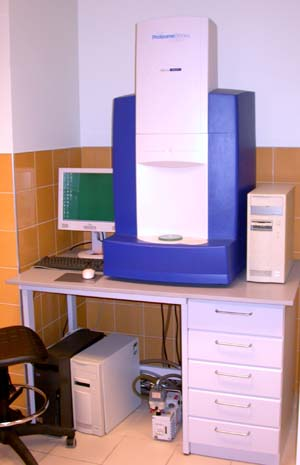
\includegraphics[width=0.6\hsize]{maldi}
% \caption{A MALDI TOF mass spectrometer.}
% \label{fig:MALDI}
% \end{center}
% \end{figure}
The MALDI technique involves embedding the large polymers of interest into a matrix of much smaller molecules, commonly acids to promote ionization during the vaporization process. 
Once the analate and matrix are co-crystallized, they are placed into a vacuum and bombarded with a laser, usually in the UV. 
The matrix is chosen to be absorptive in the range of the excitation laser, and produces a hot plume that carries the polymer of interest into the vacuum undamaged.
Once in the vacuum, the polymer can be manipulated via electric fields or optical trapping as needed.

The ability to desorb very large molecules without compromising their
integrity has many uses in biology~\cite{Hillenkamp}. 

Understanding
the statistical mechanics of such systems may help to improve current
spectroscopic techniques by providing information about other quantities,
aside from mass, that may be usefully measured. Aside from other
applications~\cite{DeutschPolyVac}, there is also the intrinsic interest
in understanding such systems. 

The dynamics of vacuum polymers has been the subject of a number of recent
investigations~\cite{Kleinert,mossa,DeutschPolyVac,DeutschCerf,Taylor,DeutschExactVac}  and show
many unusual features different from what are seen in solution. Polymers close to the coil-globule
transition show small Lyapunov exponents~\cite{mossa}. However in many situations,
the dynamics are in accord with detailed microcanonical calculations,
implying that these systems are ergodic~\cite{Taylor}. Ideal chains show
highly oscillatory time correlation functions~\cite{DeutschPolyVac}, whereas
the addition of self interactions damps these oscillations although they
are still quite pronounced for small chains~\cite{Taylor}.  Although there
is no coupling to a heat-bath, the nonlinear dynamics of these models
gives rise to an effective damping of individual monomers which is similar
to that of Kelvin damping~\cite{SethnaBookKelvinFriction}.  Adding local angular 
potentials to polymers increases this type of damping but does not
inhibit oscillations for sufficiently long chains~\cite{DeutschCerf}.

In this paper, we further investigate the equilibrium statistics
of a noninteracting polymer chain of $N$ links in a vacuum, where
energy, momentum, and angular momentum are conserved. Previous
work~\cite{DeutschExactVac} found an analytical solution for a ring
polymer with conserved angular momentum.  The average radius of gyration
as a function of angular momentum was obtained. The most
surprising feature of that calculation is that the radius of gyration when
the angular momentum is zero is less than that of a chain without that
conservation law. The radius of gyration still is proportional
to $\sqrt{N}$ but now with a different proportionality constant.

The calculation performed for a ring chain~\cite{DeutschExactVac} does not
extend easily to linear chains.  Here we use an approach that diverges considerably
from the previous one to obtain the statistics of a linear chain under
the same conditions. The new approach has some similarities to techniques used in statistical quantum mechanics~\cite{KleinertBook}In both cases, although the intermediate steps
produce rather lengthy expressions, the final answers are quite simple.
This suggests that there may be another underlying principle that can be
used to understand systems with constant angular momentum.

Aside from the average radius of gyration of such a system, there is
another important quantity that describes it, that has hitherto not
been studied. For finite angular momentum, the chain is expected to
become anisotropic, flattening in the direction of the angular momentum
vector. It is therefore of interest to calculate the average size
of a chain both perpendicular and parallel to the angular momentum.
However our analytic method is only applicable in calculating quantities
which have rotational symmetry such as the radius of gyration. It will
not work for studying chain anisotropy. Therefore we turn to numerical
methods to study this problem. We find, rather surprisingly, that the
chain continuously flattens in the direction of the angular momentum
showing universal scaling in the same rescaled variables used to
characterize the full radius of gyration. 



\chapter{Exact Solution}
Following previous work ~\cite{laliena} we begin by writing down the entropy as a function of the total energy $E$, angular momentum $L$, and number of particles $N$,  including terms for the conservation laws to be enforced. 
\begin{equation}
W(E,L,N) = C \int \delta(E - K - \Phi)\delta^{(3)}(\mathbf{L} - \sum_i \mathbf{r}_i \times \mathbf{p}_i)\delta^{(3)}(\mathbf{r}_{cm})(\prod_{i=1}^N d^3r_id^3p_i)
\end{equation}
where $K$ is the total kinetic energy and $\Phi$ the total potential energy. We are choosing a coordinate system so that
the center of mass $\mathbf{r}_{cm} = 0$.

We take the potential energy to be the elastic energy of the polymer chain and in addition include an isotropic quadratic potential that
will be used to calculate the radius of gyration. In terms of the continuous arclength $s$ dependent position variables that we will use 
below, 
\begin{equation}\label{eq:DefPhi}
\beta \Phi =  \int^{Nl}_0 \frac{3}{2l} |\frac{d \mathbf{r}}{ds}|^2 + \epsilon r^2(s)  ds 
\end{equation}
where $l$ is the chain link length, which is independent of the other properties of the chain.

Because we are taking $N$ to be large, we can convert this to a partition function, with the energy conserving delta function expanded in exponential form.
\begin{equation}
Z(\beta,L,N) \propto  \int d^3k \int e^{ i\mathbf{k\cdot L} }e^{ -\beta(K+\Phi) }e^{ -i\mathbf{k}\cdot \sum_i \mathbf{r}_i\times \mathbf{p}_i }\delta^{(3)}(\mathbf{r}_{cm})(\prod_{i=1}^N d^3r_id^3p_i)
\end{equation}

After integrating over the momenta and taking into account rotational symmetry we arrive at the form~\cite{DeutschExactVac}

\begin{equation}\label{partzeta}
Z[\beta,L,N] = \frac{c}{L} \int_0^\infty \sin(kL)\zeta(\beta,k)dk
\end{equation}
where $\zeta$ is a function of the magnitude of $k$ and inverse temperature  $\beta$ only. The constant $c$ is of no physical importance and
\begin{equation}\label{rawzeta}
\zeta(\beta,k)= \int e^{ -\int^{Nl}_0 (\frac{Tmk^2}{2l} +\epsilon)(x(s)^2 + y(s)^2)+\epsilon z(s)^2 + \frac{3}{2l}  |\dot{\mathbf{r}}|^2  ds}\delta(\mathbf{r}_{cm}) \delta \mathbf{r}(s) .
\end{equation}
Now we perform a scaling on $L$, $k$, and $s$ in order to normalize out the length of the chain and the temperature.
\begin{eqnarray}
L^\prime = \frac{\sqrt{12}}{Nl\sqrt{mT}} L\\
k^\prime = \frac{Nl\sqrt{mT}}{\sqrt{12}} k\\
s^\prime = \frac{\sqrt{12}}{Nl} s
\end{eqnarray}
The rescaling factors are based on the expected value of $L$ for the usual model without conservation of angular momentum, and produce a set of dimensionless variables. This will allow us to compare chains of all sizes and temperatures on a common scale.
After doing these rescalings, the form of Eq. \ref{partzeta} remains unchanged, and Eq. \ref{rawzeta} changes to:
\begin{equation}\label{scaledzeta}
\zeta(\beta,k^\prime)= \int e^{-\int_0^{\sqrt{12}} (k^{\prime2}/2l + \epsilon^\prime)(x^\prime(s^\prime)^2 + y^\prime(s^\prime)^2 ) + \epsilon^\prime z^\prime(s^\prime)^2  + \frac{3}{2l} |\dot{\mathbf{r}^\prime}|^2 ds^\prime}\delta(\mathbf{r}^\prime_{cm}) \delta \mathbf{r^\prime}(s^\prime)
\end{equation}
It is interesting to note that the explicit dependence on $\beta$ has disappeared and $\zeta$ is now only a function of $k^\prime$. The dependence on the total length of the chain has also been factored into $k^\prime$, but the length of the individual monomers remains.
Now we expand the center of mass conserving delta function in complex exponential form.
\begin{equation}
\zeta(k^\prime)= \int e^{-\int_0^{\sqrt{12}} (k^{\prime2}/2l + \epsilon^\prime)(x^{\prime2} + y^{\prime2} ) + \epsilon^\prime z^{\prime2}  + \frac{3}{2l} |\dot{\mathbf{r}^\prime}|^2 + i x^\prime l_x + i y^\prime l_y + i z^\prime l_z ds^\prime}  dl_xdl_ydl_z \delta \mathbf{r^\prime}(s^\prime) .
\end{equation}
These terms can be combined with the existing exponents using completion of squares which results in path independent phase factors and a constant offset to the paths, e.g. $x^\prime (s) \to x^\prime (s) + const.$ . Since all possible paths are included in the integral, the offset has no effect.

We now have a nice separation into a simple Gaussian integral and a factor that is very similar to the path integral form of a harmonic oscillator. 
\begin{equation}
(\int e^{\sqrt{12}[ -(l_x^2 + l_y^2)/4(\frac{k^{\prime2}}{2l} +\epsilon^\prime) - l_z^2/4\epsilon^\prime]}dl_xdl_ydl_z)  (\int e^{-\int_0^{\sqrt{12}} (k^{\prime2}/2l + \epsilon^\prime)(x^{\prime2} + y^{\prime2} ) + \epsilon^\prime z^{\prime2}  + \frac{3}{2l} |\dot{\mathbf{r}^\prime}|^2 } \delta \mathbf{r}^\prime)
\end{equation}
The first integrals of the $l$'s are trivially integrated but we must still perform the path integral in parentheses. 
These decouple into path integrals over the $x$, $y$, and $z$ directions and each one has an action of the form
\begin{equation}
\int_0^{\beta_0} \frac{M}{2}(\dot{x}^2 + \omega_0^2 x^2)dt .
\end{equation}
$M$ does not depend on $k$ or $\epsilon$, and $\omega_z$ has no $k$ dependence.
After making this analogy, we can see that for any two fixed path endpoints, the functional integration will give the Greens function for a thermal harmonic oscillator. To obtain a sum over all paths, we simply need to integrate the Greens function $\rho$ ~\cite{feynman} over both its arguments,
\begin{equation}
\zeta_i = \int \rho_i(x_1,x_2)dx_1dx_2
\end{equation}
where $i = 1,2,3$ represent the $x$, $y$, and $z$, path integrals respectively.
The Greens function is easily integrated and the result is 
\begin{equation}\label{eqn:zomega}
\zeta_i \propto \frac{\omega_i}{\sqrt{ \sinh{(\sqrt{12}\omega_i)}}}
\end{equation}
Putting all of this back into Eq. \ref{partzeta} we get the form for $Z$
\begin{equation}
Z(L^\prime) = \frac{c}{L} \sqrt{\frac{\omega_z}{\sinh{(\sqrt{12}\omega_z)}}} \int_0^\infty k^\prime \sin(k^\prime L^\prime) \frac{\omega}{\sinh(\sqrt{12}\omega)} dk^\prime .
\end{equation}
The radius of gyration can be expressed as
\begin{equation}
R_g^2 = -\frac{1}{Nl}\frac{\partial \ln Z}{\partial \epsilon}\vert_{\epsilon=0}
\end{equation}
The logarithmic derivative allows us to separate the factors in $Z$ and treat each as terms in a sum.
The first term is simple
\begin{equation}
\lim_{\epsilon\to0}\frac{\partial \ln}{\partial \epsilon}\sqrt{\frac{\omega_z}{\sinh{(\sqrt{12}\omega_z)}}} = -\frac{1}{18}N^2l^3
\end{equation}
The second term is more complex due to the integral, so we begin by rewriting the logarithmic derivative as a ratio.
\begin{equation}
\lim_{\epsilon\to0} \frac{\frac{\partial}{\partial \epsilon}\int_0^\infty k^\prime \sin(k^\prime L^\prime) \frac{\omega}{\sinh(\sqrt{12}\omega)} dk^\prime}{\int_0^\infty k^\prime \sin(k^\prime L^\prime) \frac{\omega}{\sinh(\sqrt{12}\omega)} dk^\prime}
\end{equation}
Since the integral is over $k^\prime$ we can pull the derivative and limit inside the integration. This simplifies the integrand considerably as $\lim_{\epsilon\to0} \omega = k^\prime/\sqrt{3}$
\begin{equation}
\lim_{\epsilon\to0} \frac{\frac{\partial}{\partial \epsilon}\int_0^\infty k^\prime \sin(k^\prime L^\prime) \frac{\omega}{\sinh(\sqrt{12}\omega)} dk^\prime}{\int_0^\infty k^\prime \sin(k^\prime L^\prime) \frac{\omega}{\sinh(\sqrt{12}\omega)} dk^\prime}  = \frac{L^\prime N^2}{6\pi l^3\tanh(\frac{L^\prime \pi}{4}) }
\end{equation}
Putting all of these pieces together we obtain our final result,
\begin{equation}
\label{eq:finalresult}
\frac{R_g^2}{Nl^2} = \frac{1}{18} + \frac{L^\prime}{6\pi\tanh(\frac{L^\prime\pi}{4})}
\end{equation}
A plot of this is shown in Fig. \ref{fig:rgplot} by the solid line. The simulation results that are also displayed will be discussed in Sec. \ref{sec:simresults}.
Note that for $L^\prime = 0$, $R_g^2/(N l^2) = (1/18) + 2/(3 \pi^2) \approx 0.1231$, which is about $74\%$ of $1/6$, the value of the same
quantity without conservation of angular momentum enforced.
\begin{figure}
\begin{center}
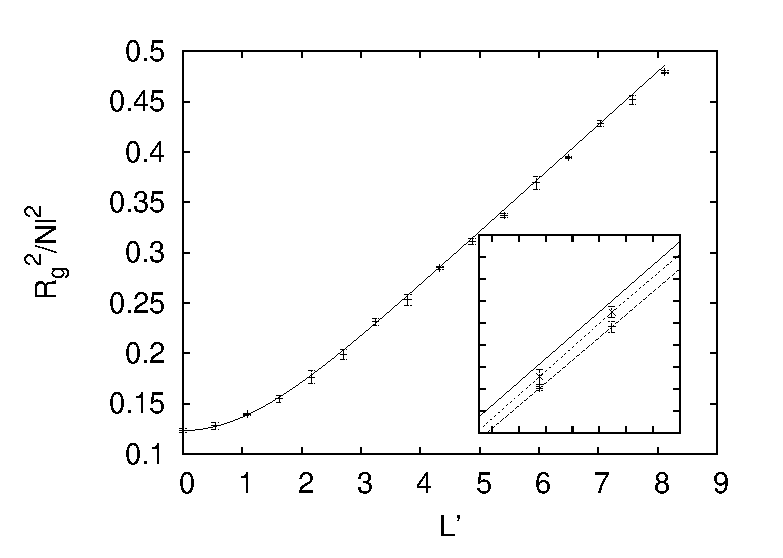
\includegraphics[width=\hsize]{radius}
\caption{Plot of $\frac{R_g^2}{Nl^2}$ along with simulation results
using a chain length $N = 128$. Inset is a section from $L^\prime=5.5$
to $L^\prime=7$ showing the exact solution as a solid line along with results from simulations done with $N = 32$ (farthest from line)
and $N = 64$. }
\label{fig:rgplot}
\end{center}
\end{figure}

For the same reason as for the ring calculation~\cite{DeutschExactVac}, for fixed $L^\prime$ and $N\to \infty$, we are permitted to take this
system to be at constant temperature, because as was discussed in detail~\cite{DeutschExactVac}, the relation between energy and temperature
has no dependence on $L^\prime$ in this limit.


\section{High $L$ limit}
In the limit of large $L$, Eq. \ref{eq:finalresult} gives $R_g^2/Nl^2 \to L^\prime/6\pi$. One would expect typical configurations at high $L$ would consist of a fairly straight line rotating rapidly around its center. The solution for the equilibrium case of constant angular velocity can be found by setting the change in tension along the chain equal to the centripetal force. This gives an equation for the position of each monomer as a function of its location along the chain, $r(s)$, for simplicity defined with $s=0$ at the center of the chain. For large $N$, the tension approaches zero at the ends of the chain.
\begin{equation}
-k\frac{d^2r}{ds^2} = m \omega^2 r \\
\end{equation}
where $k$ is the entropic elastic spring coefficient.
From this we get that $r(s) \propto \sin(\sqrt{\frac{m}{k}}\omega s)$, and that $Nl\omega/2\sqrt{k} = \pi/2$. Higher modes exist, but they double back and are expected to not be minimal free energy solutions. They are also not consistent with the straight chain model we are assuming. Using the integral definition of angular momentum
\begin{equation}
L = \frac{m \omega}{l}\int_0^{Nl}  r^2(s)ds 
\end{equation}
the radius of gyration squared is
\begin{equation}
R_g^2 \equiv \frac{1}{Nl}\int r^2(s)ds = \frac{1}{\omega m N } L = \frac{1}{\sqrt{mk}\pi}L = \frac{l}{\sqrt{3mT}\pi}L = \frac{L^\prime Nl^2}{6\pi}
\end{equation}
and therefore we see that in the limit of high $L$, our model behaves as one would expect.
\section{Partition Function}
The partition function itself can be obtained easily from Eq. \ref{eqn:zomega} by taking $\epsilon \to 0$ and performing the integration.
\begin{equation}
\lim_{\epsilon \to 0} Z = \frac{1}{L} \int k^{\prime2} \frac{\sin(k^\prime L^\prime)}{\sinh(2k^\prime)}dk^\prime = \frac{\pi^3}{32L^\prime}\frac{\tanh(L^\prime \frac{\pi}{4})}{\cosh^2(L^\prime \frac{\pi}{4})}
\end{equation}
To obtain the distribution over $L^\prime$ we need to normalize this Z, taking in to account the angular integration over the direction of $L^\prime$.
\begin{equation}
\int 4\pi L^{\prime2} Z dL^\prime = \pi^2
\end{equation}
so our normalized partition function is 
\begin{equation}
Z = \frac{\pi}{32L^\prime}\frac{\tanh(L^\prime \frac{\pi}{4})}{\cosh^2(L^\prime \frac{\pi}{4})}
\end{equation}
A plot of this is displayed in Fig. \ref{fig:P}.
This partition function can be related to the probability density in the space of angular momentum. Since $Z$ was normalized for three dimensions, it will be the three dimensional density $\rho(\mathbf{L^\prime})d\mathbf{L^\prime}$. One can simply integrate out the trivial angular dimensions to get the density in terms of the radial scalar $L^\prime$.

The distribution shows a long exponential tail into high $L^\prime$.
\begin{figure}
\begin{center}
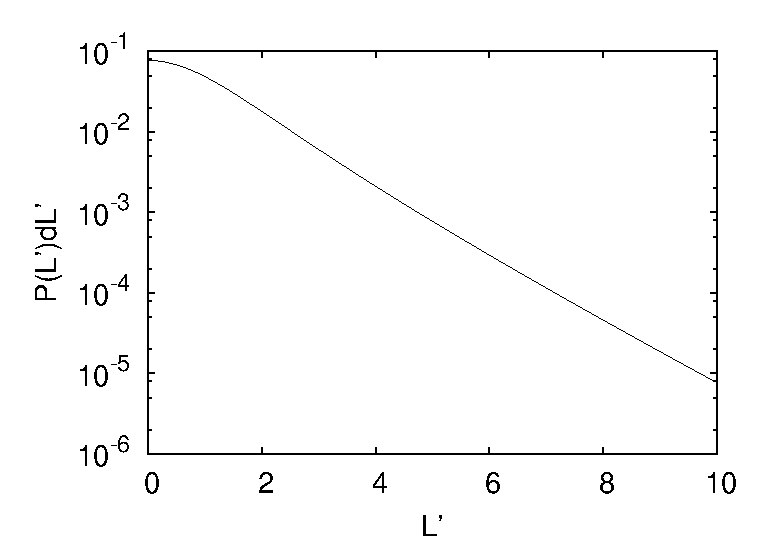
\includegraphics[width=\hsize]{P}
\caption{Plot of $P(L^\prime))$, with clear non-Gaussian behavior for high $L^\prime$}
\label{fig:P}
\end{center}
\end{figure}

\section{Simulation Results}
\label{sec:simresults}
In addition to the exact calculation, further studies were carried out using simulation. First the analytical results concerning the radius of gyration as a function of $L^\prime$ were verified. Second we were able to investigate other quantities that were beyond the means of our analytic method.

\begin{figure}
\begin{center}
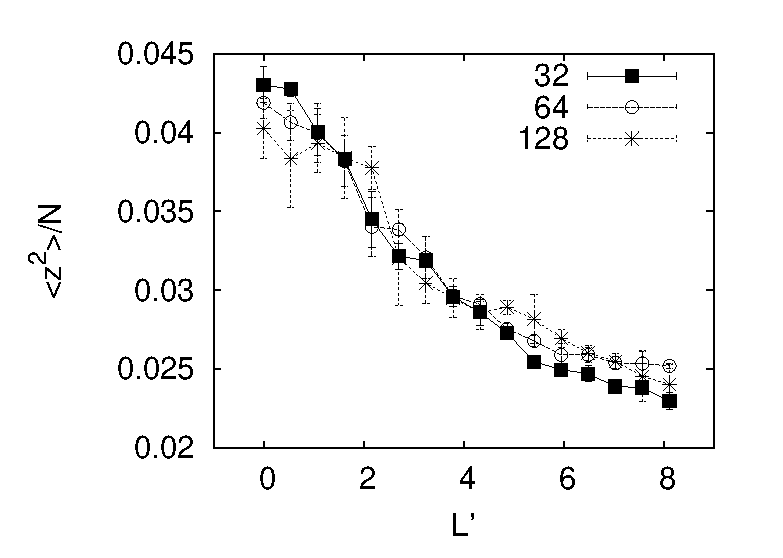
\includegraphics[width=\hsize]{zsq}
\caption{Plot of the simulated radius of gyration in the direction of angular momentum as a function of rescaled $L$, for chain sizes $N=32$,$64$ and $128$. }
\label{fig:zsq}
\end{center}
\end{figure}


We used a molecular dynamics method ~\cite{DeutschCerf} that was developed to simulate chains in a vacuum. It
consisted of freely rotating rigid links, conserving energy and angular
momentum, corresponding to a system with fixed temperature and angular momentum. Rigid links were employed to minimize problems with equilibration that are often seen with one dimensional nonlinear systems~\cite{FPU,BermanIzrailev}. The input angular momentum and the output measurements were
scaled by the total chain length for comparison. The initial values of
the angular momentum were chosen to cover a range of $L^\prime$ values, and the
angular momentum was explicitly checked and conserved during the runs.
First the simulation was compared to the theoretical results for the
normalized radius of gyration. The results of these simulations can be
seen in Fig. \ref{fig:rgplot}, and show excellent agreement with the
theoretical prediction. The main plot shows the exact result (solid line)
along with data for chains with $N=128$. The inset shows that the deviation in the asymptotic form for high
$L^\prime$ decreases as the number of simulation chain links is increased and
appears to be due to the finite size of the simulation system. The two chains lengths
used in the inset are $N=32$ and $N=64$ which are more accurate than the data
for $N=128$. They also indicate that the finite size corrections to the
analytic form are $O(1/N^\alpha)$ for some $\alpha$ of order unity, as shown in Fig. \ref{fig:scalen}.
\begin{figure}
\begin{center}
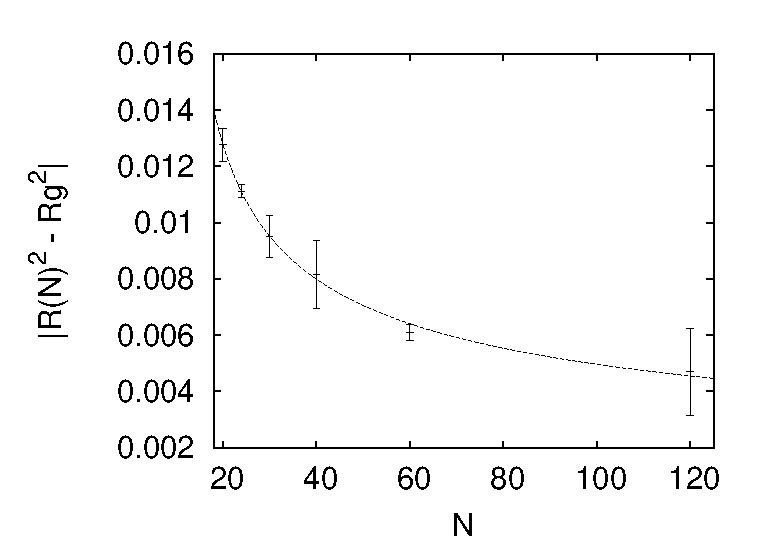
\includegraphics[width=\hsize]{scalen}
\caption{Plot of the deviations in $R_g^2$ as a function of chain size $N$. The dashed line is the best fit curve with $\alpha = 0.436$.}
\label{fig:scalen}
\end{center}
\end{figure}

For nonzero angular momentum the polymer chain is expected to become
anisotropic. The analytic methods used earlier require an isotropic
form for the quantities being averaged, causing the investigation
of the anisotropy by such means to be outside the scope of our
analysis. Therefore we turned to the simulation to explore the aspect
ratio of the polymer as a function of $L^\prime$, with the aspect ratio is defined
as $\sqrt{\langle z^2 \rangle /\langle R_g^2 \rangle}$. The aspect ratio
itself is dominated by the asymptotic linear behavior of the radius of
gyration, and displays what appears to be an inverse power law falloff
as expected. More interestingly, $\langle z^2 \rangle$ itself appears to
fall off as $L^\prime$ increases, even for low values of $L^\prime$.  This is shown in Fig. \ref{fig:zsq}  where the
vertical axis is scaled in the same manner as for the radius of gyration,
by dividing by $N$ and taking $l,m,T$ all to be unity, and the horizontal axis is $L^\prime$.  The three chain lengths seem to collapse onto one curve after the rescaling of length
and angular momentum. This is unexpected because for a ideal gaussian
chain each dimension has independent statistics, which our model should resemble for low $R_g$. The coupling should only be apparent in the limit of high $L$ where 
the rigid link model should approach a straight line solution. However
this is unlikely to be an explanation, as the straight line regime
would imply a leveling off of the radius of gyration, which is not
seen, see Fig. \ref{fig:rgplot}. Moreover, the falloff is independent of the number of chain links
in the simulation and collapsed onto a single curve, so is not likely
due to the non gaussian nature of the model. This decrease in $\langle z^2 \rangle$ is slow and
does not appear to have a nonzero asymptote, and is likely to be a low
power law or logarithmic in nature.


\section{Conclusions}

In this paper, we considered the equilibrium properties of an ideal linear chain in a vacuum
that conserves energy, momentum, and angular momentum. We were able to compute the average
radius of gyration of such a chain as a function of its angular momentum $L$. We also computed
the distribution of angular momenta for chains in thermal equilibrium. 
We verified that our analytical result for the radius of gyration is correct by performing
numerical simulation and by analyzing its asymptotic form in the limit of large angular momentum.
The derivation of this result differs from that of a ring chain but in both cases the final
result is relatively simple involving hyperbolic trigonometric functions. The underlying reason
for this is still unclear.

Our numerical simulations show that the radius of gyration perpendicular
to the angular momentum vector increases with $L$, as to be expected,
however in addition to this, the radius of gyration parallel to the
angular momentum, which we take to be in the $z$ direction, decreases.
This is very different than what a naive analysis would suggest. If we
were to go to a frame rotating at angular velocity $\Omega$, then in
thermal equilibrium (without angular momentum conservation), this is
equivalent to an additional potential $- m \Omega^2 r^2_{xy}/2$, where
$r_{xy}$ is the projection of a coordinate onto the $x-y$ plane.  For an ideal
gaussian chain, all three directions decouple and$\langle z^2\rangle$
is independent of $L$. However a more rigorous analysis based on the
approach of this paper is not equivalent to this, and it is not clear
how statistics in the $x-y$ plane and $z$ direction are coupled to cause
this effect.


\part{Biopolymers}

\chapter{Biological Motivation}
While discovering the properties of a polymer by itself is extremely useful as a foundation for understanding their behavior, polymers are rarely found in vacuum.
Polymers are often found in complex systems, with one of the most familiar examples being biology.
Biological systems make extensive use of polymers, and produce many different kinds for a variety of uses.
Some are used for structural support, some for energy storage, others can be used to store information.
A biopolymer can be any kind of polymer created or used by a biological system.
Bioplolymers can also play a less direct role in biological functions.
The structural biopolymers often pay a vital role in dynamic properties by laying the foundation on which other dynamic processes can operate.


\section{Cytoplasmic Streaming}
One of the biological processes in which the properties of polymers plays a very important role is cytoplasmic streaming. 
Cytoplasmic streaming is the flow of cellular cytoplasm, along with organelles and other materials, around the cell. 
It is usually characterized by motion over distances that would be prohibitive to traverse via diffusion alone.

While most often seen in plants, whose cell walls restrict outside perturbations of the interior fluid, the effect is seen in a wide variety of cells. 
The biological functions that this streaming accomplishes vary from case to case, whether it be for delivery of materials for focused growth or a more chaotic stirring to distribute organelles.
The driving forces behind this mass motion of cytoplasm are believed to be motor proteins carrying cargo along the cytoskelton.
The hydrodynamic drag from these cargoes, called impellers, along with the high fluid viscosity inside the cell, cause long range motion of the fluid.
This long range fluid motion can have many uses for the cell.
In some cases, materials need to be localized into specific regions, while in other cases materials need to be efficiently mixed into the entire cytoplasm.
The exact components of the streaming mechanism are still under investigation, and depend on the system in question.

\section{\emph{Drosophila} Oocyte}
The specific example of cytoplasmic streaming we studied is that found in certain stages of the development of \emph{Drosophila}, a commonly studied type of fly.
The streaming takes place during the \emph{Drosophila}'s oocyte stage, when it consists of one large cell and a few nurse cellls.
\emph{Drosophila} are extensively studied and provide a well understood basis on which to perform variations to explore the parameters involved in streaming.

In \emph{Drosophila} oocytes there are two forms of microtubule based streaming. 
First is a slow disorganized streaming, where slow localized motion of cytoplasm is thought to help distribute pattern forming determinants. 
These slow streams are rather chaotic in appearance, and do not show long range correlations across the cell.
The second type of streaming present is a fast, well-ordered motion of cytoplasm that begins just before nurse cells inject more cytoplasm into the oocyte. 
In this stage, the streaming displays correlations in direction on the size scale of the entire cell. It is believed that this fast streaming is crucial for proper distribution of material withing the oocyte.
In both of these cases, motor proteins walking along a microtubule mesh-work appear to play a vital role. 
Some examples of this type of streaming are shown in Fig. \ref{fig:streamslow}

[*** fig:streamslow ***]

\subsection{Microtubule Pathways}
Microtubules are flexible hollow polymers of tubulin subunits that
serve many critical functions in eukaryotic cells. A cartoon of the microtubule structure is shown in Fig \ref{fig:tubestruct}

\begin{figure}[htp]
\begin{center}
(a)
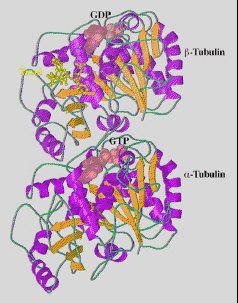
\includegraphics[width=0.45\hsize]{alphabeta.png}
(b)
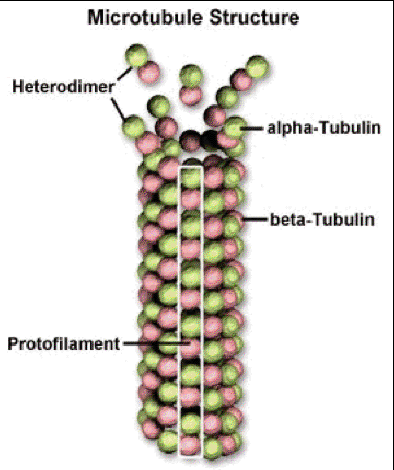
\includegraphics[width=0.45\hsize]{tubestruct.png}
\caption{
(a)
Microtubules are made out of dimers composed of $\alpha$-tubulin and $\beta$-tubulin.
(b)
The tubulin dimers form a hollow tube with either 13 or 15 linear tracks running along its length. These tracks are followed by the molecular motors as they walk along the microtubule.
Images courtesy of Bill Saxton.
}
\label{fig:tubestruct}
\end{center}
\end{figure}
They are utilized
in structural contexts, because of their relatively stiff, yet flexible,
mechanical properties.  They also act as directional highways through the
viscous cytoplasm. Molecular motor proteins carry cellular constituents
along the microtubules with kinesin moving toward their fast growing
``plus-ends" and dynein moving toward their slow growing ``minus-ends".
Many studies have focused on motor driven transport processes that
generate asymmetric distributions of specific cytoplasmic constituents;
asymmetries that are essential for complex cellular functions. 

\begin{figure}[htp]
\begin{center}
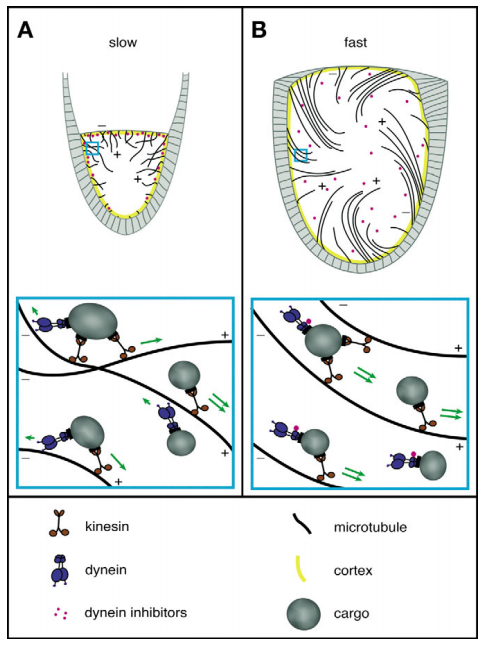
\includegraphics[width=0.5\hsize]{biomodel.png}
\caption{ 
A speculative model for fast streaming in \emph{Drosophila} oocytes, care of Bill Saxton et al. 
(A) During the slow streaming stage, microtubules are not aligned and only small scale motion is observed. 
(B) During the fast streaming stage, microtubules are see in correlated into long dynamic arrays. 
The lower panels show expanded views of the boxes shown in the upper panels. 
}
\label{fig:biomodel}
\end{center}
\end{figure}


It is not only important to understand the mechanism at work during the streaming itself, but also in the mechanisms used to control the timing of that streaming phase.
The large scale streaming requires the correlated effort of a significant fraction of the motors involved, so it is possible that small changes in system parameters could cause a transition between slow and fast streaming.


\subsection{Components of Mixing}

% We will analyze a surprising role for microtubules and kinesin in cytoplasmic streaming that has evolved to accomplish just the opposite; efficient homogeneous mixing of the contents of a cell~\cite{SerbusSaxton} and see there Supplemental Movie 13~\cite{Movie13}.

Vigorous streaming is is observed during the final stages of
development of {\em Drosophila} oocytes which serves to disperse asymmetrically
distributed mRNA particles, protein complexes, and membranous
organelles.  The mixing process is important for subsequent
embryonic development, and cannot be accomplished by
diffusion alone.  
The fluid viscosity is quite high and, on the size scale of the cell, the organelles are actually rather large. 
This gives a diffusion timescale that is far to long to be effective for biological processes. 
For example  a $ 1\mu m$ yolk-filled vesicle in
the cytoplasm, assuming a viscosity 8 times that of water ~\cite{LubyPhelps}
would take approximately a week to diffuse the $500 \mu m$  length
of an oocyte. This is far too long to satisfy the need for the mixing
of yolk-filled oocyte cytoplasm with the mass of yolkless nurse
cell cytoplasm that floods the anterior of the oocyte near the
end of its development.

The problem of mixing in small systems, such as in microfluidics
chambers, has been the subject of much investigation ~\cite{Squires}. The
way that a fluid at low Reynolds number is stirred has a
profound effect on the efficiency of homogenization. For
example,  the steady state flow fields generated by a single
stirrer inside a closed chamber are far less efficient than
the more chaotic flows generated when  several stirrers are used~\cite{Aref,Aref2000}.
Rigorous analyses in two dimensions show that mixing is
most efficient when topological chaos is created by three or more
stirrers, as can be shown by application of the Thurston-Nielsen
classification theorem~\cite{Thurston,Fathi,Handel}.  With this in mind, it is
interesting to note that during fast cytoplasmic streaming in
{\em Drosophila} oocytes, microtubules appear to be locally aligned
along dynamically changing curved paths that produce travelling
waves~\cite{SerbusSaxton}.  
The streaming cytoplasmic fluid moves along those paths, in patterns reminiscent
of flowing water and seaweed.

During fast streaming, yolk particles in the
cytoplasm are observed to have a speed of roughly $0.25 \mu m/s$.  The particles
within a region stream for the most part in one direction,
but with a non-negligible deviation in that direction over
time. The fluctuating directions, which parallel the curved paths of
the microtubules in the same region, serve to stir cytoplasm
in a chaotic manner that, as the preceding paragraph suggests,
is important for efficient mixing.

At first sight, it might appear that the time-dependent wave-like
motion is due to turbulence of the surrounding fluid. However at the low Reynolds found in this system
numbers, inertial effects are negligible and turbulence is
impossible~\cite{BergRandomWalksinBiology}. Therefore one is left with a mystery of
the relationship of fluid and filament and
how such chaotic patterns could come about. The plus-end
directed motor kinesin-1 plays a crucial role in this, as
shown by 
genetic mutations in its force producing subunit (Khc)  that prevent streaming and mixing~\cite{SerbusSaxton}.
The speed of unloaded kinesin along the microtubule has been
measured to be in the $0.5 ~-~ 1 \mu m/s$ range~\cite{SvobodaBlock,MeyhoferHoward}.  This is higher
than the fluid speeds measured during fast cytoplasmic streaming~\cite{SerbusSaxton}
and is also consistent with the role of kinesin in powering
the mixing.
Inhibition of the opposing minus-end directed motor protein,
dynein, has a complementary effect,
actually stimulating fast cytoplasmic streaming ~\cite{SerbusSaxton}.  Microscopy studies
suggest that microtubules participating in this motion have their
minus ends attached to the cortex and their plus ends away from
the cortex in the interior of the oocyte~\cite{SerbusSaxton,ChaSerbus}.  

The explanation
that we analyze for the streaming phenomena is very simple: the
mass motions of cytoplasm and the microtubule undulations are complementary
physical consequences of kinesin moving cargo 
toward the plus ends of microtubules whose minus ends
are in contact with the cortex. The cargoes serve as impellers that
both drive the fluid motion away from minus-ends and generate
tangential forces that move plus-ends toward minus-ends causing
bends in the microtubules. This has been suggested previously to
explain cytoplasmic streaming, but without a physical model of the
mechanism~\cite{SerbusSaxton}. The analysis below shows that long range hydrodynamic
forces couple individual impellers, resulting in an effective
mechanism for drag-induced bulk movement of cytoplasm.  We then
show that an instability in the dynamics leads to chiral symmetry breaking giving rise to
wave-like motion of microtubules, and show that the time and length scales
predicted are in good agreement with the previous experimental
results.

%Mixing Paper
\chapter{Single Polymer Dynamics}

\section{Microtubules and Molecular Motors}
Consider impellers to be objects each with maximum linear dimension
$a$, and with a mean spacing of $d$ arranged in a straight line along the microtubule, as shown in Fig ~\ref{fig:spheres}. 

\begin{figure}[htp]
\begin{center}
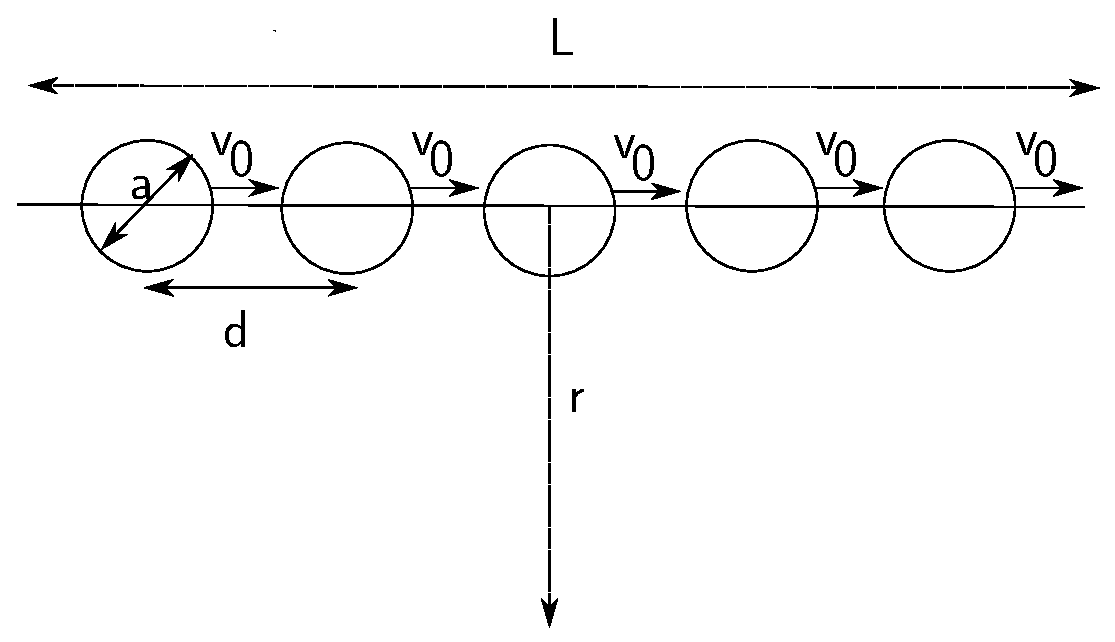
\includegraphics[width=\hsize]{spheres.eps}
\caption{ 
A train of spherically shaped impellers of diameter $a$ and separation $d$, all moving in a fluid with a velocity $v_0$.
The fluid velocity is measured at a point a distance $r$ from the axis.
}
\label{fig:spheres}
\end{center}
\end{figure}

These impellers are pictured as spheres, but hydrodynamics is not sensitive to
the exact shape of an impeller, as it depends mainly on its maximum linear dimension~\cite{BergRandomWalksinBiology}. 
We will
now analyze the amount of streaming due to motion of these impellers
moving on a single microtubule. We initially consider the impellers to be much larger than
the kinesin molecules so that they dominate the hydrodynamical response
of the fluid.

If spherical impellers were close-packed along the microtubule, that is $a \approx
d$, then this problem would be equivalent to a single rod of length $L$
moving at constant velocity $v_0$ in the fluid in a direction parallel
to its long axis.  In that case, the velocity field for distances
$r \ll L$ has only a weak logarithmic dependence of $r$, meaning that up
to a correction of order $\ln(L/a)$, the velocity field is only weakly
dependent on distance and of order $v_0$. (Here we take the velocity of the fluid
to go to zero far from the rod.)
This is related to the well
known result that the drag on a rod of length $L$ is of the same order
as that of a sphere of diameter $L$ despite the latter's much greater volume~\cite{BergRandomWalksinBiology}. Such a system of densely packed impellers would
be very efficient at driving fluid motion and only a low density of microtubules
would be needed for cytoplasmic streaming.

Now consider the more realistic case in which the impeller size is less than
the spacing between them, which is much less than the length of a
microtubule, that is $a < d \ll L$.  At a distance $r \gg d$, the
velocity field will behave just as in the closed-packed case except appear
to have a diminished impeller velocity. That is for $d \ll r \ll L$,
the magnitude of the velocity $v(r)  = v_0 f(a/d) g(r)$, where $g(r)$
contains all the distance dependence of the velocity field, and $f(a/d)$
is how the velocity scales with the ratio of $a/d$. In the limit where
$a/d$ is very small, the system becomes dilute and the velocity between 
impellers will decay to zero. We recover the motion of isolated impellers
in this case, where it is well known (e.g. Stokes' drag) that the velocity
field is proportional to $a$. Therefore for small argument $x$, $f(x)$ is
linear (in other words, the fluid velocity is proportional to $a$.) 

Using this general argument we conclude that, independent of the exact shape of the impellers,
the flow velocity is reduced from the closed-packed case by a factor $\sim a/d$. The effect
of the impellers only starts decreasing substantially at a distance of order the
length of the microtubule $L$, below which it should only have a weak logarithmic
dependence. In other words, for a spherical region just enveloping a microtubule,
the fluid velocity is slowly varying and reduced from the kinesin motor velocity 
by a factor of order $a/d$.

\section{Enhancement of Streaming Due to Hydrodynamics} 

As we have seen, there are actually many microtubules in these cells. To understand how this
affects the above analysis, consider all space filled with an infinite forest of them all oriented
in the same direction. 

%%% Begin new explaination
Let us assume that the microtubules and impellers have managed to set up fast streaming and the fluid now has a long range global velocity $v$.
Because they are tethered at one end, the microtubules are stationary in this configuration, and as such the net force on them must be zero. 
This means that the hydrodynamic drag on a section of microtubule must be exactly balanced by the other forces acting on that segment.
There are two other forces acting on the segment; the kinesin and the neighboring segments.
\begin{equation}
\label{eq:mfnetMforce}
b_M v = \frac{\partial}{\partial s}T(s) + F_k
\end{equation}
Where $b_M$ is the local drag coefficient of the segment of microtubule, which can be approximated to within logarithmic corrections as that of a sphere with radius equal to the segment length, therefore in an fluid of viscosity $\eta$, $b_M = 6\pi \eta d$

We also know that the same force balance must hold for the impellers, with their drag force relative to their fixed velocity. 
However, they don't have connections between neighbors so there is no tension term. 
Their force balance is 
\begin{equation}
\label{eq:mfnetIforce}
b_I (v - v_0) =  -F_k
\end{equation}
Where $b_I$ is the local drag coefficient for the impellers, with $b_I = 6\pi\eta a$.

The force exerted on the fluid is simply opposite of the drag terms. It is important to note here that these two equations are for forces acting in slightly different locations, as one is for the microtubule segment and the other for the impeller. 
We will go on later to show that this small separation (on the order of the length of the kinesin), will give rise to a quadrapole like term in the fluid motion.
This term falls off as $1/\br^3$ and should not have significant effect on the long distance fluid motion.
For considering the long range flow field of the fluid, it is safe to neglect these terms and for now treat these two force equations as happening at the same location.
The total force acting on the fluid per unit length is then:
\begin{equation}
\label{eq:mfnetFforce}
b_I (v - v_0) + b_M v = -\frac{\partial}{\partial s}T(s)
\end{equation}
The equality to the gradient of the tension will be useful in simulating the fluid motion later, as the tension is determined by the configuration of the microtubule directly. 
In the more general case, all of the forces that act directly on the microtubule would be present on the right hand side of this equation, while the forces due to the kinesin cancel out.

To determine the value of the fluid flow speed, we need to find the long range fluid velocity due to the force densities supplied by the microtubules and impellers.
Since the microtubules and impellers are assumed to fill all of space, we can treat their effect as a uniform force density applied to the fluid.
The fluid velocity field due to an applied local force is proportional to the force and falls of as $1/r$. If we integrate this over a region of linear dimension $R$, we get that the flow velocity is
\begin{equation}
\label{eq:mfflow}
v = \int -\kappa \frac{(b_I (v - v_0) + b_M v)}{|\br|} d^3\br = -2\pi \kappa R^2 (b_I (v - v_0) + b_M v)
\end{equation}
Where $\kappa$ is proportionality constant determined by the fluid interaction strength which will not effect the final result of this analysis.
Solve this for $v$
\begin{equation}
\label{eq:mfflowsol}
v = \frac{2\pi \kappa R^2 b_I}{2\pi \kappa R^2(b_I + b_M) + 1} v_0
\end{equation}
And now take the limit as the total system size goes to infinity
\begin{equation}
\label{eq:mfflowlimit}
\lim_{R\to\infty} v = \frac{b_I}{b_I + b_M} v_0 = \frac{a}{a+d} v_0
\end{equation}
The second equality comes from the fact that the drag coefficients are proportional to the maximal linear dimensions of the objects in question. 
In this case $a$ for the impellers, and $d$ for the segment of microtubule. 
Because of this, we expect $b_M > b_I$ because the impellers must be able to fit along the microtubule.

This result makes good intuitive sense, as we would expect the fluid velocity to be some form of weighted average between the velocities of the two classes of objects in contact with it. 
It also has the nice limit that if the drag from the microtubule were to be small, the fluid would move at the walk speed of the kinesin, and that if the drag from the microtubule were to be very large, the fluid velocity would be greatly suppressed but never quite zero.
In the case of exact symmetry between the two lengths, the fluid velocity becomes halfway between the walk speed and zero, as one would expect.

The exact result will depend on the shape of the impellers, and the local fluid velocities near the microtubule impeller system will of course be more complex than a constant uniform flow field.
%%%end old explanation


%%% Begin old explanation
% First if we ignore the microtubules and just consider the spherical impellers, then
% if we move to a reference frame moving with the impeller velocity, the system is static
% and the velocity everywhere is zero. Therefore in the original reference frame, the
% fluid is also moving uniformly at the impeller velocity. This is not correct because
% we have ignored the hydrodynamic drag of the microtubules represented by the line going through
% the spheres in Fig. \ref{fig:spheres}. To estimate their effect on the fluid velocity, 
% denote the drag coefficient on an impeller by $b_I$ and that of a section of microtubule length $d$ by $b_M$. Then
% we go to a reference frame velocity $v$ such that the total force acting on the combined system of
% impellers and microtubules is zero, so that $b_I(v_0 - v) - b_M v = 0$, or $v = b_I v_0/(b_I + b_M)$.
% Because the net force acting on this system is zero in this frame, $v$ is the velocity
% of the fluid far from the microtubules.
% Because within logarithmic corrections, the drag coefficients are proportional to the maximal
% linear dimensions, then a conservative estimate of
% this speed is of order $v_0 a/d$. The exact formula depends on the shape of
% the impellers. This argument assumes an infinite volume of
% microtubules but the corrections to this due to the finite nature of the system
% are not important for the estimates we are making.

%%%end old explanation

The identities of impellers in this system are still unknown but there are many possible
candidates. Anything with  large linear dimensions in at least one direction 
will give a large hydrodynamic radius $a$~\cite{BergRandomWalksinBiology}. The
other requirement is that it can attach to kinesin.  In fact
it is possible that the impellers in this situation could themselves be microtubules that are
not attached to the cortex~\cite{WangRiechmann,Seeger}.
Experimental estimates of the cytoplasmic streaming velocity
are approximately $0.25 \mu m/s$, about $\frac{1}{4}$ to $\frac{1}{2}$ the typical velocity of a kinesin
molecule. This suggests that $a/d$ is $\frac{1}{4}$ or greater.
For example, if we take the maximum dimensions of an impeller to be $250 nm$,
this predicts a spacing between impellers of $1 \mu m$ or less.

Another important biological issue is the necessity to have some microtubules in direct physical contact
with the cortex of the
oocyte, for example by tethering or by frictional forces. A free floating microtubule with kinesin moving on it will apply {\em zero} net force
to the fluid. This is a simple consequence of Newton's third law, or equivalently, conservation
of momentum. 
Contact with the cortex is crucial as it allows for transfer of force from outside of
the oocyte to the cytoplasm, enabling fast streaming of the bulk to be powered by a much smaller volume of kinesin driven
impellers.
This does not contradict
the fact that bacteria are able to swim: the force propelling the bacterium forward is
countered by an equal and opposite force on the environment, leading to velocity fields that
are dipolar at large distances. Unlike the case analyzed above, this will not lead to long range hydrodynamic motion
of the fluid and will not lead to efficient cytoplasmic streaming by relatively few motor proteins. 

%\section{Travelling Wave Instability of Microtubules}

% We now show how the kinesin generated tangential forces on microtubules give rise to travelling wave conformations 
% and calculate their angular and spatial frequency.
% A microtubule has a configuration $\br(s)$ parameterized by 
% an arclength $s$ and, at long enough length scales, can be modeled as being inextensible, 
% that is $|\partial \br/\partial s| = 1$
% with an elastic bending constant $C$. The inextensibility is enforced by a position dependent tension $T(s)$. 
% There is also a force acting on the microtubule as a result of kinesin walking along it.
% The magnitude of the force is proportional to the local speed and the size of the kinesin-driven impeller
% and the direction of the force is tangent to the microtubule,
% which, we will see, has the effect of making it buckle. We denote this with a force per unit length of $f_k$. 
% We also include a force due to the cytoplasm streaming at a velocity $v_s$ which
% we take to be in the $\hat k$ direction away from the minus end and this force tends to straighten the microtubule. This leads to the equation
% \begin{equation}
% \label{eq:microtubule}
% \nu \frac{\partial \br}{\partial t} =  -C \frac{\partial^4 \br}{\partial s^4} + \frac{\partial}{\partial s}(T(s)\frac{\partial \br}{\partial s}) -
% f_k \frac{\partial \br}{\partial s} + \nu v_{s}{\hat k} .
% \end{equation}
% where $\nu$ is a hydrodynamic drag coefficient per unit length. 

% \begin{figure}[htp]
% \begin{center}
% 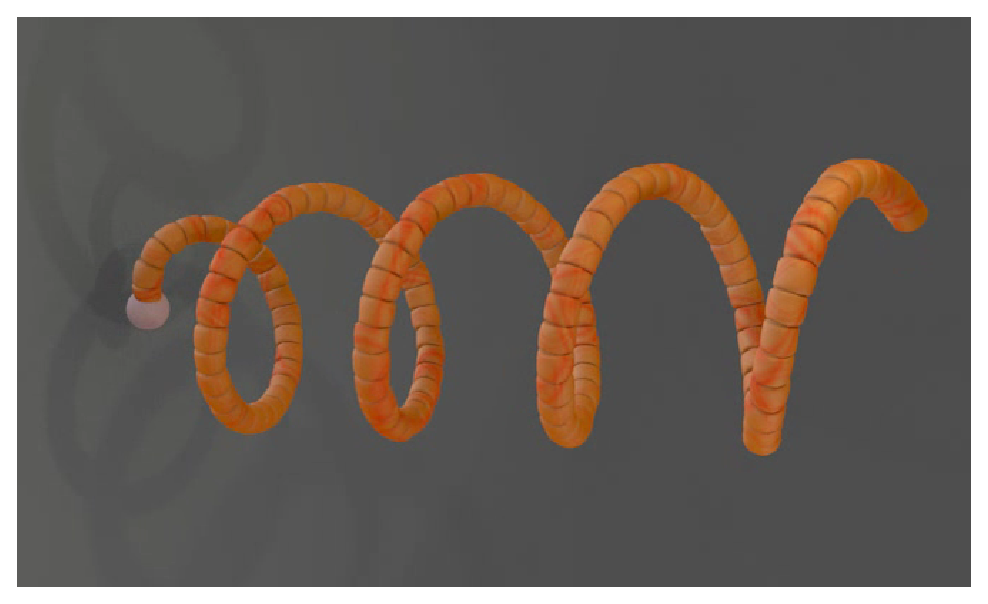
\includegraphics[width=\hsize]{simulation1.eps}
% \caption{ 
% The motion of a microtubule with a constant force being applied tangent to its axis. 
% A constant velocity in the horizontal direction  from left to right has also been applied representing
% the background from cytoplasmic streaming. The white ball on the left represents
% the point at which the microtubule's minus end is tethered. See supplemental
% movie 1~\cite{SupplMovies}. In a real oocyte, the radius of curvature would
% correspond to approximately $40 \mu m$ and the dimensions of the entire figure are
% roughly comparable to the oocyte. The thickness of the microtubule has been magnified
% by a factor of about $2000$ to facilitate viewing.
% }
% \label{fig:simulation}
% \end{center}
% \end{figure}


% We first implemented this equation numerically for a range of parameters
% and enforced boundary conditions that tethered the minus end against the cortex, while
% the plus end was free. Starting from random initial conditions, the equation rapidly goes to a steady state that
% typically is described by a curve that asymptotically becomes helical for large $s$ and rotates uniformly at constant
% angular velocity. The results of a steady state configuration are shown in Fig. \ref{fig:simulation}. 
% The supplemental movies~\cite{SupplMovies} discussed below, show microtubule solutions for different
% parameters.
% Supplemental movie 1 shows the full time dependence~\cite{SupplMovies}. The chirality of the helix depends on its initial conditions.
% Therefore the direction of rotation is random but stable once steady state is reached.

% As the microtubule is made longer, the angular velocity and radius of the helix go to
% a constant limit. However the tethered part is not helical but nevertheless rotates
% in synchrony with the rest of the microtubule. These dynamics we analyzed in detail
% (see the supplemental information) to find the form of the solution to this equation.
% In particular we show that this equation supports travelling waves and find the
% relationship between the angular velocity of rotation $\omega$ and the asymptotic
% radius of the helix, and the external velocity fields $v_s$. In the case where $v_s = 0$, the
% relationship simplifies to 
% \begin{equation}
% \label{eq:Romega}
% \nu R \omega/f_k = 1.
% \end{equation}
% independent of chain length.

% It is interesting to note that for travelling waves, solutions can be at any scale. There is a continuous family of solutions
% all with the same shape but different scale factors. In the case of a helix, many different radii $R$ are solutions to
% these equations.

% What determines the value of $R$ that is selected? As with other problems in pattern formation such as the ``geometric model"~\cite{Kessler}
% or the full dendrite problem~\cite{Barbieri}, it is the boundary conditions
% that are responsible for the unique value of $R$ that is selected. In this case, the microtubule minus end is tethered, $\bu(0) = 0$
% but the plus end is free.
% The solution will only exist for discrete values
% of $\beta \equiv C/(R^3 f_k)$. Numerical analysis gives, $\beta = 0.05 \pm 0.0005$. 
% This implies that 
% \begin{equation}
% \label{eq:R}
% R =  (C/(\beta f_k))^{1/3}.
% \end{equation}

%%%INSERT MATH PAPER

%Single chain math Paper
\section{Motion of Microtubule With Kinesin Walkers}

% Here we study the motion of microtubules in the context of cytoplasmic
% streaming in stage 10B-11 Drosophila oocytes.  At that stage, the roughly
% hemispherical oocyte is bounded by a plasma membrane and an underlying
% cortex comprised of an actin filament meshwork.  Long microtubules,
% with minus ends attached to the cortex, have their plus ends free.
% Kinesin-1 motor proteins that walk along the microtubules toward plus
% ends generate opposing forces on the microtubule and the surrounding
% viscous cytoplasm.  Cytoplasm is thus moved toward plus ends, generating
% vigorous flows for mixing.  Because minus ends are anchored, the equal
% but opposite force on a microtubule generates dynamic bending along
% its length.  The results of this work have been used to understand this
% phenomenon in recent work by the authors~\cite{DeutschBrunnerSaxton}.
\label{sect:MathAnalysis}
We begin with the equation for a microtubule with an applied force tangent to the direction of chain. The position
of the microtubule at arclength $s$ and at time $t$ is denoted $\br(s,t)$. As is usual at small scales, all inertial effects are negligible
and the system is dominated by the drag coefficient per unit length $\nu$,
\begin{equation}
\label{eq:microtubule}
\nu \frac{\partial \br}{\partial t} =  -C \frac{\partial^4 \br}{\partial s^4} + \frac{\partial}{\partial s}(T(s)\frac{\partial \br}{\partial s}) -
f_k \frac{\partial \br}{\partial s} + \nu v_{s}{\hat k} .
\end{equation}
$C$ denotes the elastic bending constant of the microtubule. The tension $T(s)$ enforces the inextensibility of microtubules which
can be written as  $|\partial \br/\partial s| = 1.$ 
\begin{figure}[htp]
\begin{center}
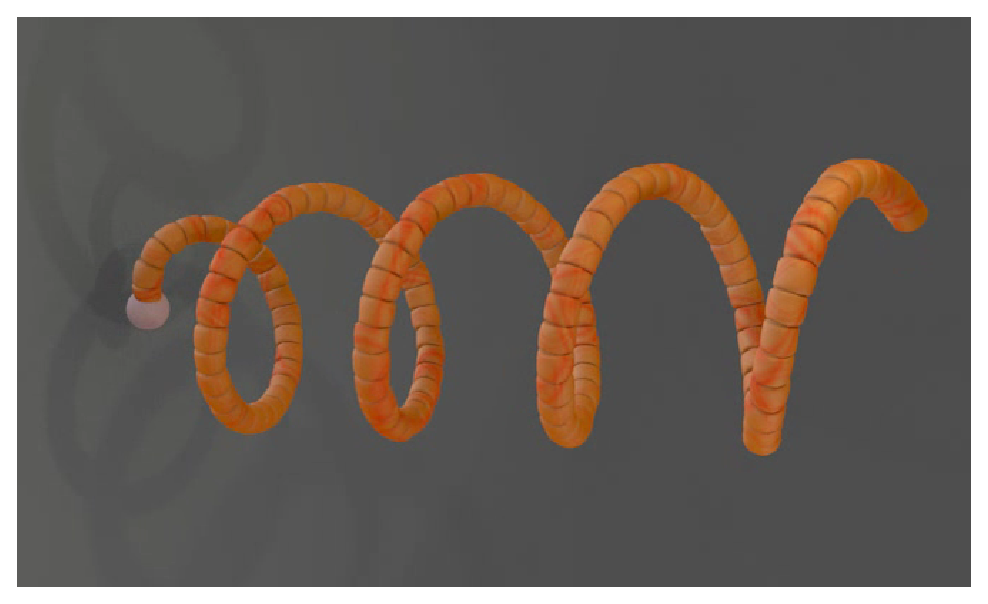
\includegraphics[width=\hsize]{simulation1.eps}
\caption{ 
The motion of a microtubule with a constant force being applied tangent to its axis. 
A constant velocity in the horizontal direction  from left to right has also been applied representing
the background from cytoplasmic streaming. The white ball on the left represents
the point at which the microtubule's minus end is tethered. See supplemental
movie 1~\cite{SupplMovies}. In a real oocyte, the radius of curvature would
correspond to approximately $40 \mu m$ and the dimensions of the entire figure are
roughly comparable to the oocyte. The thickness of the microtubule has been magnified
by a factor of about $2000$ to facilitate viewing.
}
\label{fig:simulation}
\end{center}
\end{figure}
Kinesin motors walking along the microtubule are assumed to be carrying cargo that acts as an impeller pushing the surrounding
cytoplasmic medium. By Newton's third law, this force produces a drag on the impellers that transmits this force to the
attached microtubule. Assuming a high density of kinesin walkers, the effective force on the microtubule will be in the
direction of the local tangent to $\br(s)$ which is $\partial \br/\partial s$. The coefficient $f_k$ gives the strength of the force.
Lastly we add a uniform flow field representing the velocity of the cytoplasm $v_s$ in the vicinity of the microtubule
which we take to be in the $\hat k$ direction.

We rescale to dimensionless variables 
\begin{equation}
\label{eq:rescale}
\sigma = s/\rho_0,~ \bu = \br/\rho_0, ~ \tau = t \omega_0,  ~ T' = T \rho_0^2/C, ~{\rm and} ~ h = \nu v_s/f_k 
\end{equation}
so that
\begin{equation}
\label{eq:dimensionless}
\frac{\partial \bu}{\partial \tau} =  - \frac{\partial^4 \bu}{\partial \sigma^4} + \frac{\partial}{\partial \sigma}(T'(\sigma)\frac{\partial \bu}{\partial \sigma}) -
\frac{\partial \bu}{\partial s} + h {\hat k} .
\end{equation}
This requires that 
\begin{equation}
\label{eq:scaling}
\omega_0 = f_k/(\nu \rho_0), ~  {\rm and} ~ \rho_0^3 = C/f_k. 
\end{equation}
$\rho_0$ and $\omega_0$ are constants that make our new variables dimensionless.

We will consider solutions where one end (the {\em minus} end) is tethered to a point, say the origin, so that
$\br(s=0,t) = 0$ and is freely hinged at that point. The other end is free.
The total arclength of the microtubule is denoted by $L$.
The general characteristic of all numerical solutions to Eq. \ref{eq:microtubule} is that
for large $s$ the solutions appear to be traveling waves. In fact, the form of solution
becomes independent of $L$ so in fact we could consider this problem in the limit $L\rightarrow \infty$.
For example we find solutions that asymptotically become helical with a fixed path and radius for
large $s$. Other solutions are planar and are periodic in $s$. In all these cases the solution
has the form of a travelling wave that we analyze in detail below.

\section{Steady State Travelling Wave Solutions}

Now we look for steady state travelling wave solutions. First we clarify what this means.
The whole microtubule should not be translating because one end, (far away from where
the travelling wave solution is valid) is tethered. 
The position averaged over one period of a monomer, $\langle u \rangle$, should be  time independent.
If the microtubule is stretched out
in one particular direction, there should be a displacement $\bu_d$ of the microtubule about a straight
line solution,
\begin{equation}
\label{eq:travelling}
\bu(\sigma, \tau) = \bu_d(\sigma-v\tau) + \alpha \sigma {\hat k}.
\end{equation}
The term $\bu_d$ describes a displacement that travels along the backbone of the chain maintaining its shape.
Therefore we require
\begin{equation}
\label{eq:ud_constraint}
\frac{\partial \langle \bu_d \rangle}{\partial \sigma} = 0
\end{equation}

Substituting Eq. \ref{eq:travelling} into Eq. \ref{eq:dimensionless} gives a left hand side
of $-v \partial \bu_d/\partial \sigma$ and a term of the form $-\partial \bu_d/\partial \sigma$ on
the right hand side. Choosing $v = 1$ and in addition $\alpha = h$, we are left with

\begin{equation}
\label{eq:reduced_steadystate}
\frac{\partial^4 \bu}{\partial \sigma^4} + \frac{\partial}{\partial \sigma}(T'(\sigma)\frac{\partial \bu}{\partial \sigma}) = 0.
\end{equation}
We define $\bw = \partial \bu/\partial \sigma$  and
note that the inextensibility requirement $|\partial \br/\partial s| = 1$ implies that $|\bw| = 1$. We can write 
\begin{equation}
\label{eq:bw=bd_alpha}
\bw  = \frac{\partial \bu_d}{\partial \sigma} + \alpha {\hat k}
\end{equation}
Note that $\bw(\sigma,\tau)$ depends only on $\sigma -\tau$. Because $\bw$ is a function
of only one variable $\xi \equiv \sigma -\tau$, 
we can 
integrate Eq. \ref{eq:reduced_steadystate} with respect to $\xi$ obtaining
\begin{equation}
\label{eq:sphericalmotion}
\frac{d^2 \bw}{d \xi^2} - T'(\sigma)\bw = -g {\hat k}.
\end{equation}
The integration constant on the right hand side $-g {\hat k}$ must lie in the $\hat k$ direction by symmetry.
This is the same equation as that of the classical mechanics of a particle of unit mass, with position $\bw$ travelling on the surface of a 
unit sphere under the influence of gravity, with the variable $\xi$ being analogous to time. The term $-T'$ is a normal
force that constrains the particle to stay on the sphere's surface.

From Eq. \ref{eq:ud_constraint} and Eq. \ref{eq:bw=bd_alpha} we see that the motion is subject to the
constraint
\begin{equation}
\label{eq:alpha_constraint}
\langle \bw \rangle = \alpha {\hat k}
\end{equation}
The constant $g$ and the initial conditions of the particle must be chosen so as to satisfy this constraint.
There is an infinite number of solutions satisfying these conditions leading to different 
steady state solutions for the microtubule.

The spherical pendulum Eq. \ref{eq:sphericalmotion} has been analyzed~\cite{CushmanBates} in detail. In general
the orbits will not be closed, but we will relegate
our discussion below to two cases where this is the case, circular motion in Eq. \ref{eq:sphericalmotion}, corresponding to helical
conformations of a microtubule, and motion in the $x-z$ plane, corresponding to solutions similar in shape to cycloids.

\subsection{Scale Invariant Family of Solutions}
\label{subsec:ScaleInvariance}

One important point to notice about the general structure of Eq. \ref{eq:sphericalmotion} is its invariance under
change of $\xi$, that is $\xi \rightarrow \lambda \xi$. A change in scale of $\lambda$ does not modify the
solution, because $T'(\xi)$  and $g$ are both constraints, and can therefore be chosen arbitrarily. So that if
$\bw(\xi)$ is a solution to Eq. \ref{eq:sphericalmotion}, so is $\bw(\lambda \xi)$. Furthermore all solutions
of this form will have the same $\langle \bw \rangle$ and hence the same $\alpha$. Note that a length scale
shift of $\bw = \bw_0(\lambda \xi)$ corresponds to a displacement of $\bu = (1/\lambda)\bu_0(\lambda \xi)$, which
changes scale because of the $1/\lambda$ prefactor in this expression. This means that for every
steady state conformation of the microtubule, there exists a family of steady state solutions with identical
shape but arbitrary size.

\subsection{Circular Orbits}
\label{subsec:CircularOrbits}

Circular orbits are solutions to Eq. \ref{eq:sphericalmotion}. Eq. \ref{eq:alpha_constraint} requires that the vertical
height of the orbit be at $w_z = \alpha$. Therefore the radius perpendicular to $\hat k$ (the $w_x, w_y$ plane) is 
\begin{equation}
\label{eq:w_perp_alpha}
w_\perp \equiv \sqrt{1-\alpha^2}. 
\end{equation}
It is first easiest to analyze this by direct analogy to the classical mechanical problem of a unit mass particle moving on a unit sphere (the
spherical pendulum).
If the height above the sphere is $\alpha$, then application of Newton's laws gives that the tension must balance the force
of gravity $g$ and the centripetal acceleration $v^2/w_\perp$ giving
\begin{equation}
\frac{g}{v^2} \equiv \frac{\alpha}{1-\alpha^2} 
\end{equation}
Where $v$ is not the real velocity of the microtubule but $|d \bw_\perp/d\xi|$. This is the rate at which the
tangent vector rotates in the $x-y$ plane. 
Because $|d\bu_d/d\xi|  = |\bw_d| = r_c$ is a constant, $\bw_d$ is a circle. 
Therefore according to Eq. \ref{eq:travelling}, this will give a helical conformation of the microtubule. 


In the spherical pendulum analogy, the angular velocity of the particle
is $\Omega_p = v/w_\perp$. The total arclength of the chain (in dimensionless units) of a single period of
the chain is
\begin{equation}
\label{eq:SRalpha}
S = \frac{2\pi R}{\sqrt{1-\alpha^2}}
\end{equation}
and $S \Omega_p = 2 \pi$ so that $S = 2\pi/\Omega_p = w_\perp/v$. Comparing this with Eq. \ref{eq:SRalpha}
we obtain 
\begin{equation}
R = \frac{w_\perp}{v} \sqrt{1-\alpha^2}. 
\end{equation}
Using Eq. \ref{eq:w_perp_alpha} this gives 
\begin{equation}
\label{eq:Ralpha_v}
R = \frac{1-\alpha^2}{|\frac{d w_\perp}{d \xi}|} = \frac{1-\alpha^2}{v}
\end{equation}
Because $g$ is a free parameter, $v$ can be any positive number and therefore Eq. \ref{eq:Ralpha_v}
implies that the radius of the helix can be arbitrary. 

Because the velocity of this travelling wave is unity, the spatial and temporal periodicities are equal. 
Therefore the period of rotation of the helix $P'$ is equal to  $S$ in Eq. \ref{eq:SRalpha}, in the dimensionless units that we are using.
Therefore the relationship between the period and the pitch is
\begin{equation}
\label{eq:Pdimensionless}
P' = \frac{2\pi R}{\sqrt{1-\alpha^2}}
\end{equation}
In terms of our original units the period is
\begin{equation}
\label{eq:T_circle}
P = \frac{2\pi R \nu}{f_k \sqrt{1-\alpha^2}}
\end{equation}

\subsection{Two Dimensional Solutions}
\label{subsec:2dsolns}

We now consider orbits in the $x-z$ plane. This corresponds to a pendulum swinging around vertically through the bottom of the sphere.
This is a standard introductory mechanics problem. Letting $\theta$ denote the angle with respect to the $-{\hat k}$ direction,
\begin{equation}
\label{eq:pendulum}
\ddot{\theta} = -g \sin\theta 
\end{equation}
where the dots that normally represent a time derivative are really derivatives with respect to $\xi$. Low energy solutions
where the total energy $E$ is less than $g$ give $\theta$ oscillating between two bounds. 
In this case the curve for the microtubule will look sinusoidal. Beyond the separatrix where $E > g$, $\theta$ will
increase without bound. This gives rise to microtubule conformations that look close to prolate cycloids. In other words,
the microtubule forms a travelling wave that periodically loops backwards. This is shown in Fig. \ref{fig:prolate}

\begin{figure}[htp]
\begin{center}
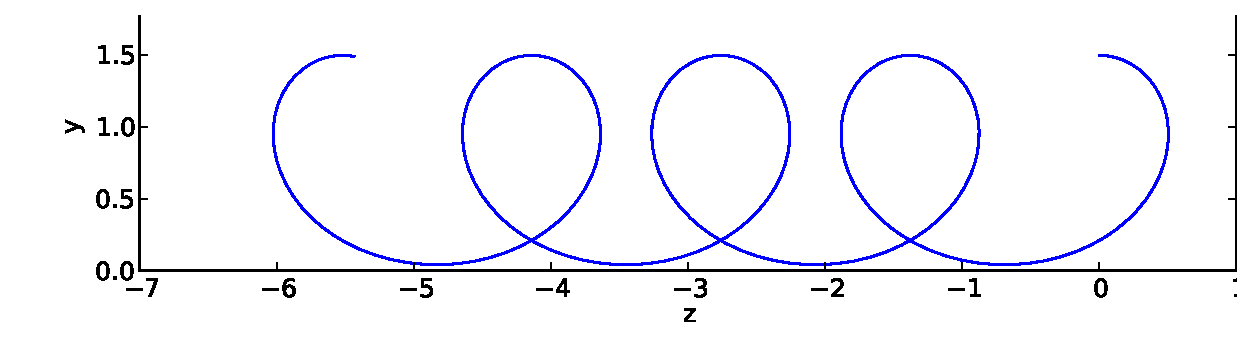
\includegraphics[width=\hsize]{shape1.eps}
\caption{ 
A two dimensional travelling wave solution for a microtubule that looks close to a prolate cycloid but
differs from it in functional form.
}
\label{fig:prolate}
\end{center}
\end{figure}

Small values of $|\alpha|$ correspond to low values of $g/E$. In this case, the particle spends almost
equal times at all points on the circle giving a small value of $\langle w\rangle = \alpha$. As $g/E$
increases to $1$, $\alpha$ increases and the loops become tighter; a situation that is very costly energetically.
However this is not the only solution to these equations for a fixed value of $\alpha$. If instead we
consider solutions with $E < g$, then large $g/E$ corresponds to small oscillations of $\bw$ about $-{\hat k}$.
In this case, $|\alpha|$ is close to $1$ and the curve has no tight loops. The shape of the microtubule
is close to a sine wave.

To obtain the relationship between $G \equiv g/E$ and $\alpha$ we use conservation of energy
to obtain the period $T$,
\begin{equation}
\label{eq:pendulumenergy}
\dot{\theta} = \sqrt{2E(1+G\cos\theta)}
\end{equation}

The time average of $\bw$ in the $\hat k$ direction is
\begin{equation}
\label{eq:avependulumcostheta}
\langle \cos\theta\rangle = \frac{\int_0^\pi \frac{\cos\theta}{\sqrt{1+G\cos\theta)}} d\theta}{\int_0^\pi \frac{1}{\sqrt{1+G\cos\theta)}} d\theta}
\end{equation}
This can be expressed in terms of elliptic integrals as
\begin{equation}
\label{eq:avecosthetaElliptic}
\langle \cos\theta\rangle =  \frac{1}{G} (1- (1+G) \frac{{\sf E}(2G/(1+G))}{{\sf K}(2G/(1+G))})
\end{equation}
Where  $\sf E$ and $\sf K$ are the complete Elliptic integrals of the first and second kind respectively.
For bounded orbits, below the separatrix, the corresponding expression can be calculated giving
\begin{equation}
\label{eq:avecosthetaEllipticBounded}
\langle \cos\theta\rangle =  -2 \frac{{\sf E}(\frac{e+1}{2})}{{\sf K} (\frac{e+1}{2}) }) + 1
\end{equation}
A plot of the $\alpha = \langle \cos\theta\rangle$ versus $1/G = E/g$ is shown in Fig. \ref{fig:AlphaVsE}
using these two expressions.
$\alpha \rightarrow 0$ in the limit as $G \rightarrow 0$. Note that there are two possible values of
$E/g$ corresponding to one value of positive $\alpha$.

\begin{figure}[htp]
\begin{center}
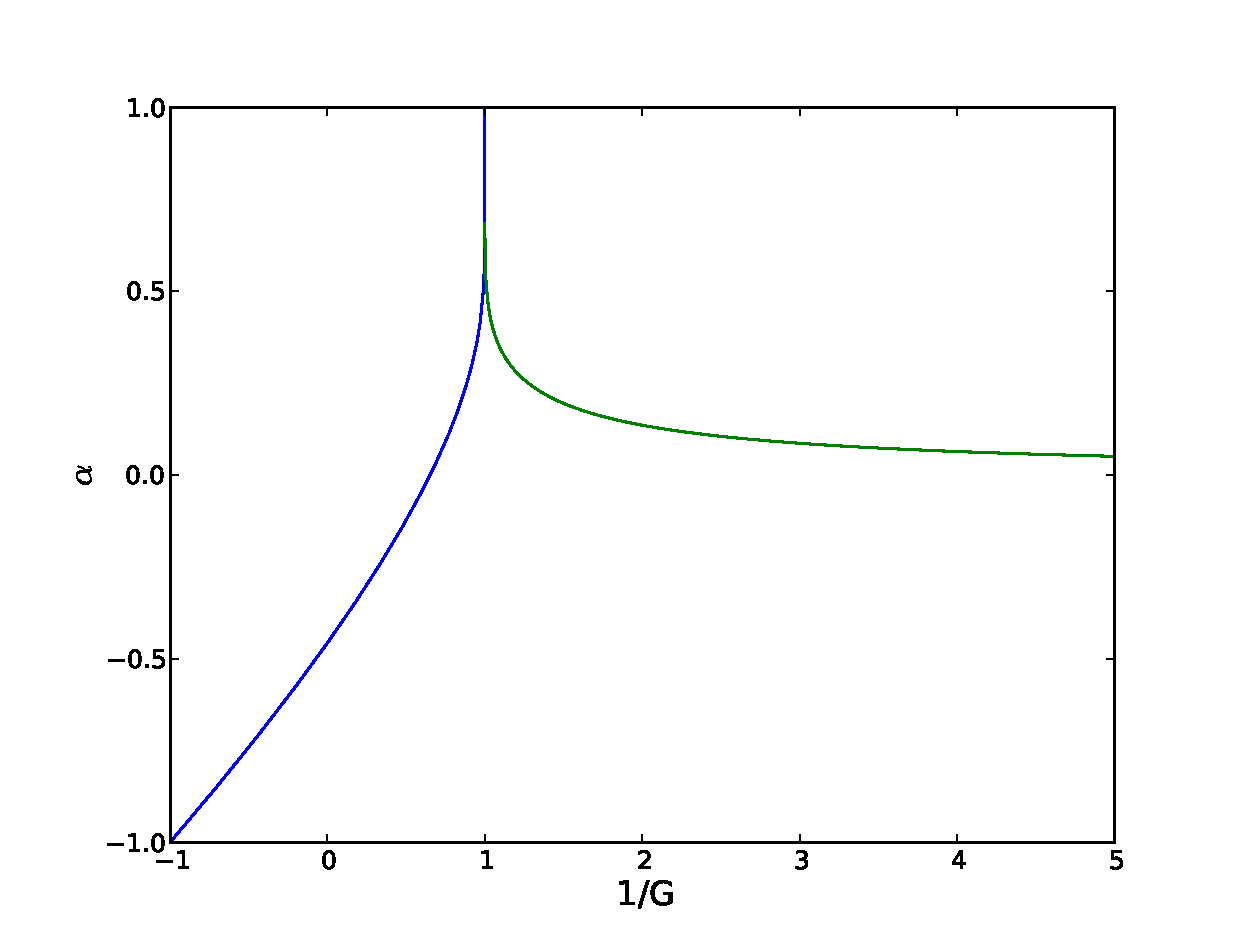
\includegraphics[width=\hsize]{alpha_vs_E.eps}
\caption{ 
A plot of the value of $\alpha$ as a function of $1/G$.
}
\label{fig:AlphaVsE}
\end{center}
\end{figure}



The case of $\alpha = 0$
corresponds to the case of circular orbits discussed in Sec.  \ref{subsec:CircularOrbits}. 
The cytoplasmic streaming velocity is $\propto h$ (see Eq.  \ref{eq:dimensionless}).
When $h = 0$, we have shown that the solutions are circular. If $h$ is now made very
small, we expect that the solution will only be slightly perturbed from circular
solutions. This corresponds to a small value of $g/E$. Therefore the value of
$G$ that is chosen for small enough $h$ should correspond to the larger value of
$1/G$ shown in Fig.  \ref{fig:AlphaVsE}. This corresponds to almost circular loops
shifting slightly forward after every turn. As $h$ increases the loops become
tighter giving rise to a high elastic bending energy. At some point therefore, 
we expect a transition to another state. In fact, simulations discussed in Sec. \ref{subsec:CompWithSims} show that near a
flat surface, the microtubule transitions out of the plane to a helical shape 
at $h \approx .385$ for $128$ links in a chain. For
still larger $h$, the microtubule becomes flat again looking close to sinusoidal.

\section{Numerical Implementation of the Full Solutions}

By comparing the steady state solutions found above for large arclength $s$ and  time $t$, we will
see that these solutions are physically realistic ones to consider. As we will see, the full
equations of motions go to solutions of this type. However this is not a complete
description of the problem, because of these solutions
a particular one is selected from a whole family of solutions. The same behavior occurs
in other problems in pattern selection such as dendritic growth~\cite{Kessler,Barbieri}.

\begin{figure}[t]
\begin{center}
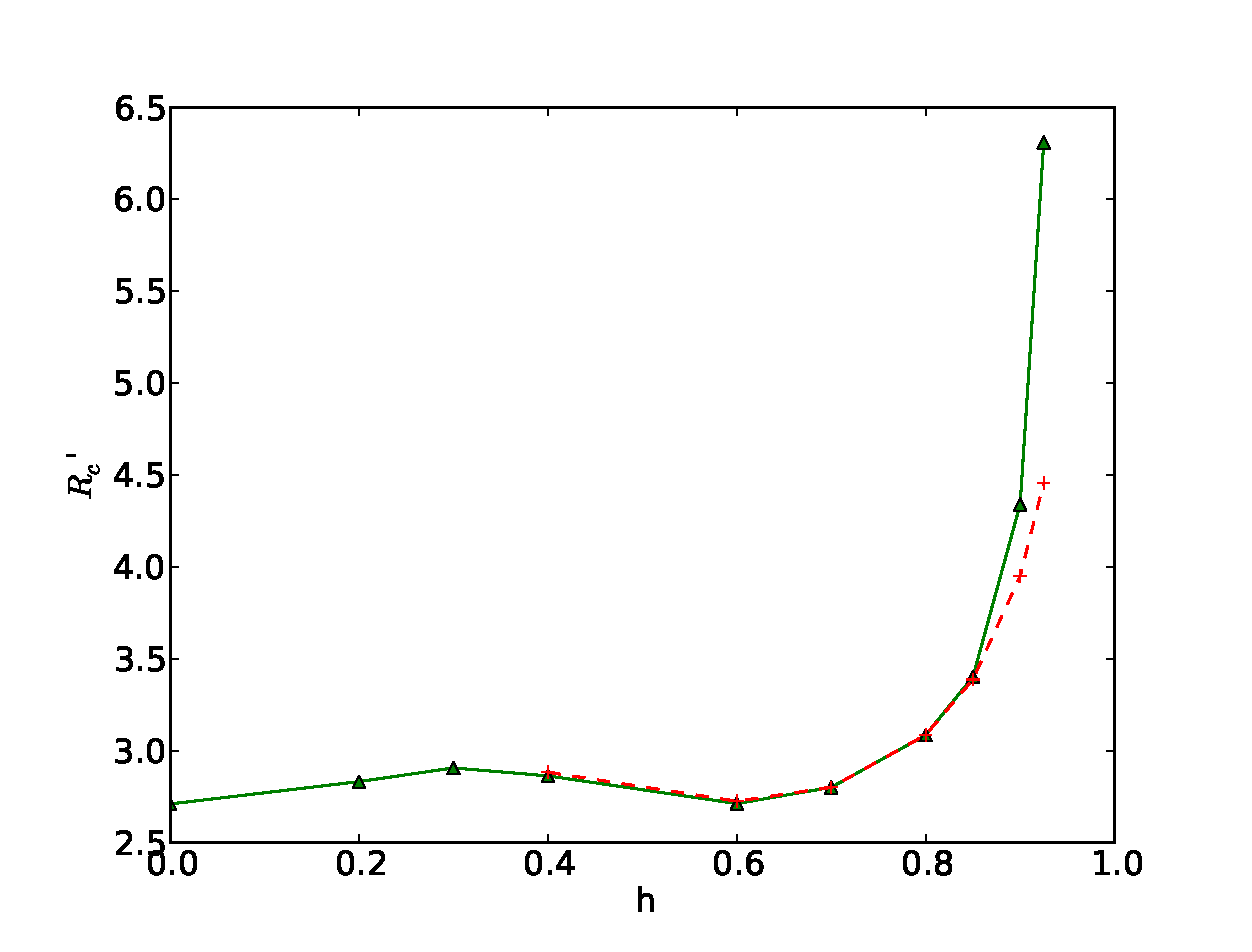
\includegraphics[width=\hsize]{rad_curv_vs_h.eps}
\caption{ 
The rescaled radius of curvature $R_c/\rho_0$ versus the rescaled velocity field $h=\alpha$.
The green triangles are for $64$ link chains, the red $+$ symbols are for chains of $128$ links.
}
\label{fig:RadCurvVSh}
\end{center}
\end{figure}

\subsection{Comparison With Simulation}
\label{subsec:CompWithSims}

Eq.  \ref{eq:microtubule} was analyzed numerically using a method similar to that
used in the context of gel electrophoresis~\cite{DeutschElectrophoresisScience,DeutschMadden}.
Link length drift was handled using a similar procedure to that implemented for chains with inertia~\cite{DeutschCerfFriction}
One end was constrained to have coordinates at the origin, while the other was free. 

A Runge Kutta time step was $0.001$, with the elastic bending coefficient $C = 20$, the kinesin force magnitude $f_k = 2$ and simulations were performed with $N=64$ or $N=128$ links,
as will be noted below.

We first consider the case of a microtubule with no wall or other external forces aside from the external velocity field.
As a function of the rescaled external velocity field $h$, the radius of curvature and period were calculated once the
system had reached steady state. Using rescaled variables as defined by Eqs. \ref{eq:rescale} and \ref{eq:scaling} we
can write the dimensionless radius of curvature as $R_c' = R_c/\rho_0$, and the dimensionless period as $P' = \omega P$.
The radius of curvature was calculated at the middle of the chain to reduce finite size effects.
The results are shown in Figs.  \ref{fig:RadCurvVSh} and \ref{fig:PeriodVSh}. The data for $R_c$, Fig. \ref{fig:RadCurvVSh} using
$64$ links, is very close to those of $128$ links except for the highest $h$ values. The data for the period, Fig. \ref{fig:PeriodVSh}(a)
show good agreement for both chain sizes at all values of $h$ studied.

\begin{figure}[htp]
\begin{center}
(a) 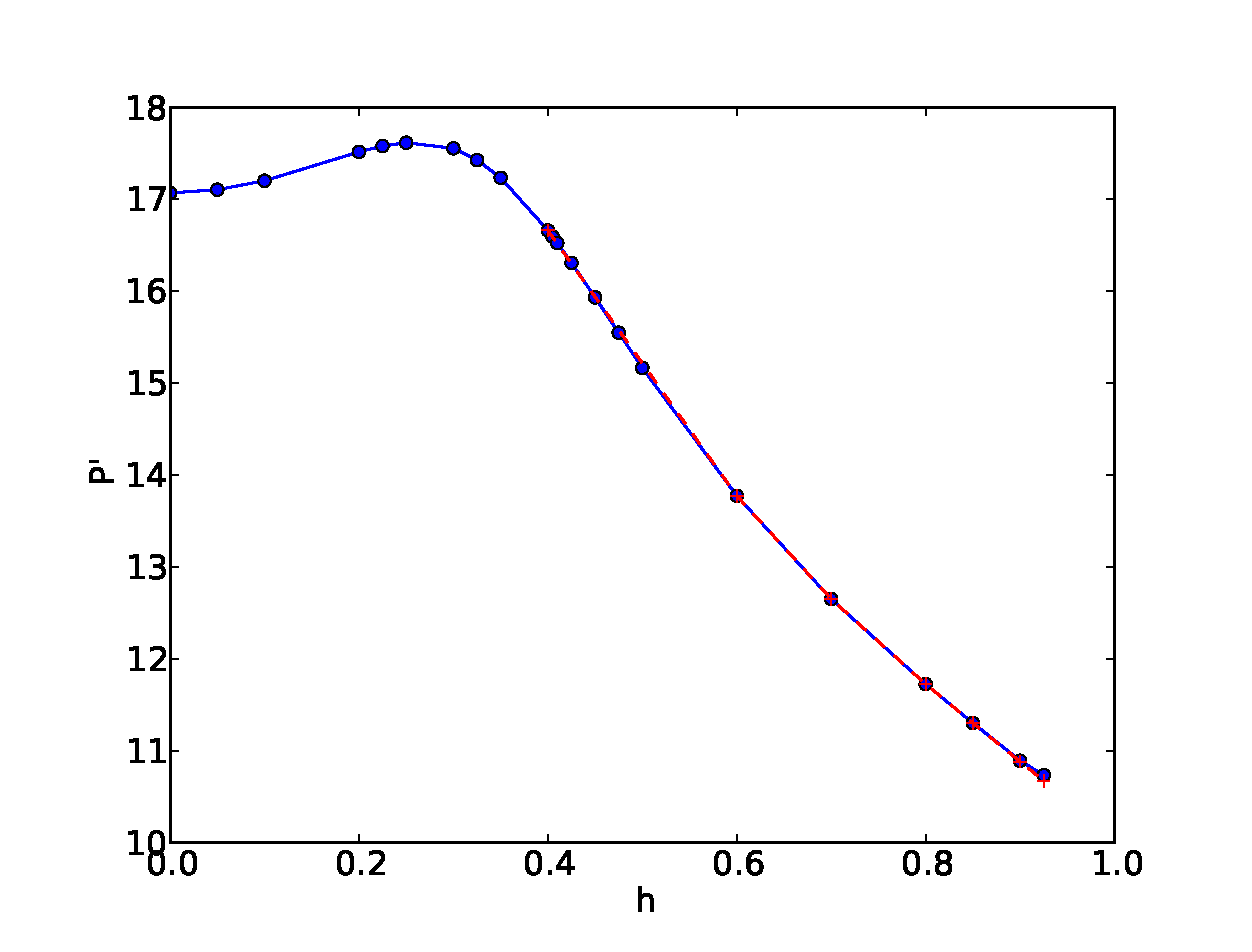
\includegraphics[width=0.45\hsize]{period_vs_h.eps}
(b) 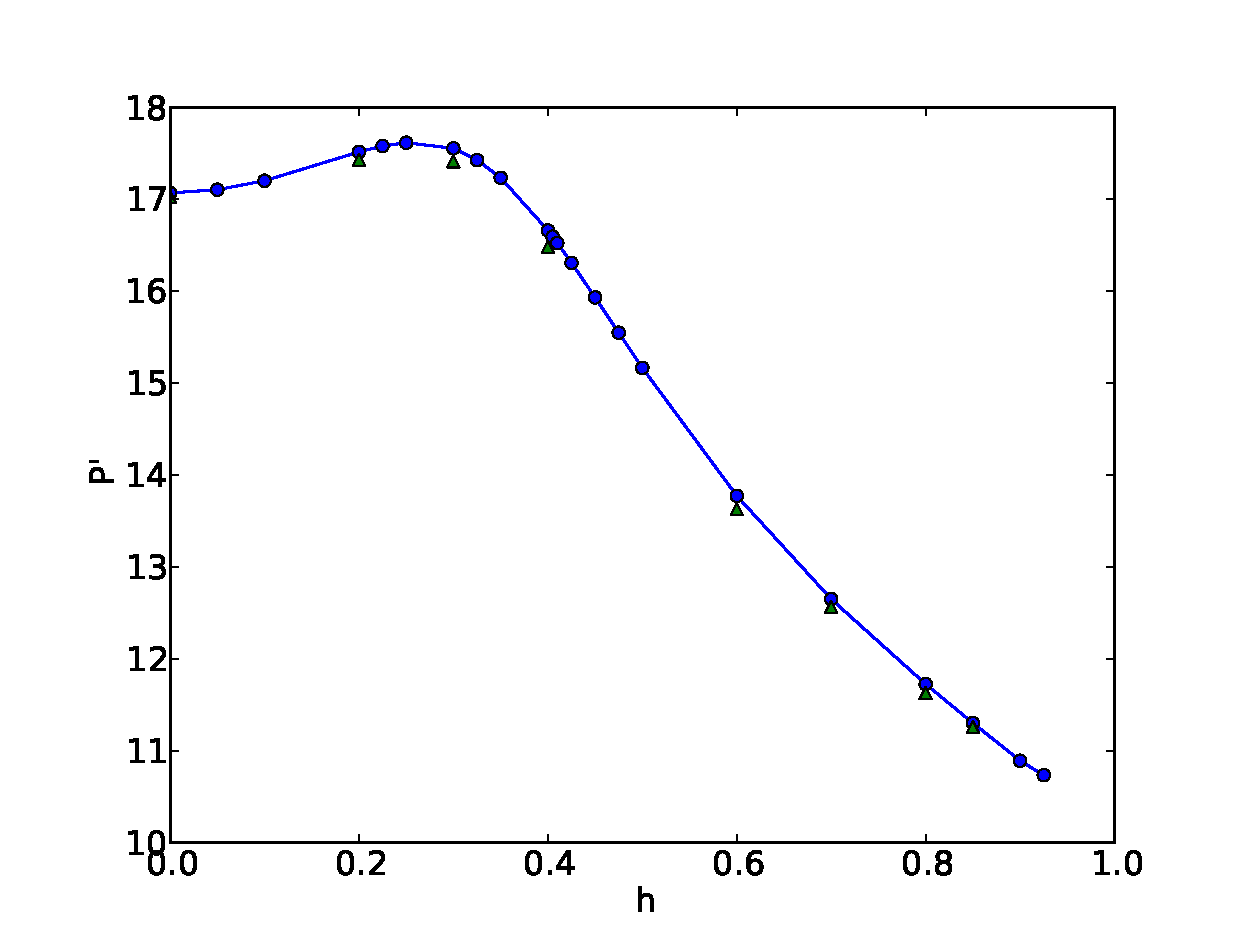
\includegraphics[width=0.45\hsize]{compare.eps}
\caption{ 
(a)The rescaled period $P' = P\omega$ versus the rescaled velocity field $h=\alpha$.
The blue circles are for $64$ link chains, the red $+$ symbols are for chains of $128$ links.
(b)
The rescaled period $P' = P\omega$ versus the rescaled velocity field $h=\alpha$
calculated by using Eq. \ref{eq:PvsRc} and data on the radius of the helix versus $h$ shown
in Fig. \ref{fig:RadCurvVSh}. The result is shown by the green triangles. 
The blue circles are the same data shown in Fig. \ref{fig:PeriodVSh} by directly
measuring the period. 
}
\label{fig:PeriodVSh}
\end{center}
\end{figure}




We now test the analytic predictions that we made relating the period to the radius of the helix and $\alpha$
given by Eq. \ref{eq:Pdimensionless}, and our conclusion that $\alpha = h$. The relationship between the
radius of curvature $R_c$ and the radius $R$ of the helix is readily calculated to be $R = R_c (1-\alpha^2)$.
Therefore Eq. \ref{eq:Pdimensionless} gives
\begin{equation}
\label{eq:PvsRc}
P' = 2 \pi R_c' \sqrt{1-\alpha^2}
\end{equation}
With this prediction and using the data for $R_c$ in Fig. \ref{fig:RadCurvVSh}, we can independently calculate $P'$ for $64$
link chains. We can only do this where finite size effects are not important and therefore omit the highest two $h$ values
from this analysis. The data, Fig. \ref{fig:PeriodVSh}(b), show excellent agreement to within the differences expected by finite size effects. This
corroborates our analytical analysis of steady state solutions. 

The case of $h = \alpha = 0$ displayed in Fig.  \ref{fig:RadCurvVSh} can be written in terms of the original
dimensional variables of Eq. \ref{eq:microtubule} using Eq.  \ref{eq:scaling}
\begin{equation}
\label{eq:Romega}
\nu R \omega/f_k = 1.
\end{equation}
And using our numeric solutions we can obtain.

\begin{equation}
\label{eq:R}
R_c =  (C/(\beta f_k))^{1/3}.
\end{equation}
From the numerical solution, this gives $\beta = 0.05 \pm 0.0005$. This is useful in analyzing experimental data, as
$R_c$ is nearly constant for $h < 0.7$.

Next we consider the presence of a wall. We introduced a force representing a wall in the $y-z$ plane of the form
\begin{equation}
\label{eq:wallforce}
{\bf f}_w =  \frac{x^2}{(x+1)^2} { \hat  i}  
\end{equation}
which is only present for $x < 0$. The force is singular at $x=-1$ preventing the chain from crossing that plane.
The period as a function of $h$ is shown in Fig. \ref{fig:WallPeriodVSh} for $C=20$ and chains with $128$ links.
\begin{figure}[htp]
\begin{center}
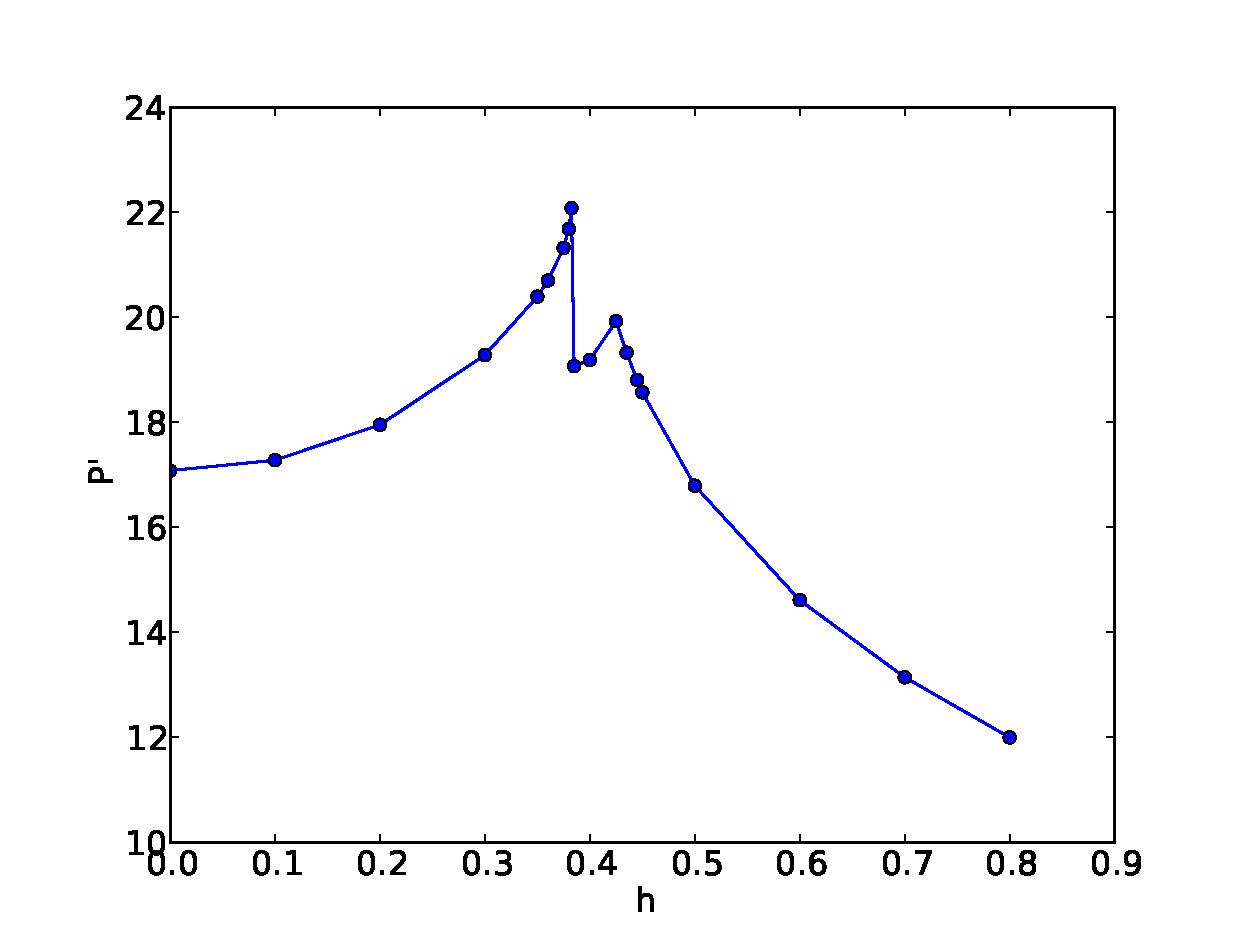
\includegraphics[width=\hsize]{wall_per_vs_h.eps}
\caption{ 
The rescaled period $P' = P\omega$ versus the rescaled velocity field $h=\alpha$
for chains of $128$ links.
}
\label{fig:WallPeriodVSh}
\end{center}
\end{figure}

For small values of $h$, the period does not vary much. The shapes obtained are flat and
appear to be the same as those found in \ref{subsec:2dsolns}. However there is non-analytic behavior at $h \approx 0.385$
corresponding to a transition to flattened helical waves. Then at $h \approx 0.425$ the solution becomes almost
completely flat and showing waves that look closer to sine waves, corresponding to the flat 
sinusoidal-like solutions studied in \ref{subsec:2dsolns}.

We now consider the dependence of period and curvature on the length of chains $L$. Our
analytical solutions have been in the limit that the chain length $L\rightarrow \infty$.
For finite length chains, we expect corrections to this behavior. This is important
to analyze in relationship to experiments using microtubule gliding assays~\cite{ValeSchnappEtAl}, which will be disussed later.
In this case we consider $h=0$ and study how the rotating spiral wave solutions vary with increasing
length. Fig. \ref{fig:RvsL}(a) shows the dependence of the radius of curvature measured
halfway along the arclength, as a function of chain length. As usual, the rescaled dimensionless
variables, see Eqs. \ref{eq:rescale} and \ref{eq:scaling} have been used. The curve
shows a non-monotonic dependence on $L$ that levels off at $L \approx 20$. 
Fig. \ref{fig:RvsL}(b) shows that the rescaled period is slightly non-monotonic as well but decreases to a constant
value at $L \approx 15$. In comparison with gliding assays, we took~\cite{DeutschBrunnerSaxton} $L = 14.0$, where
values of parameters are within $3\%$ of their asymptotic values.


\begin{figure}[htp]
\begin{center}
(a)
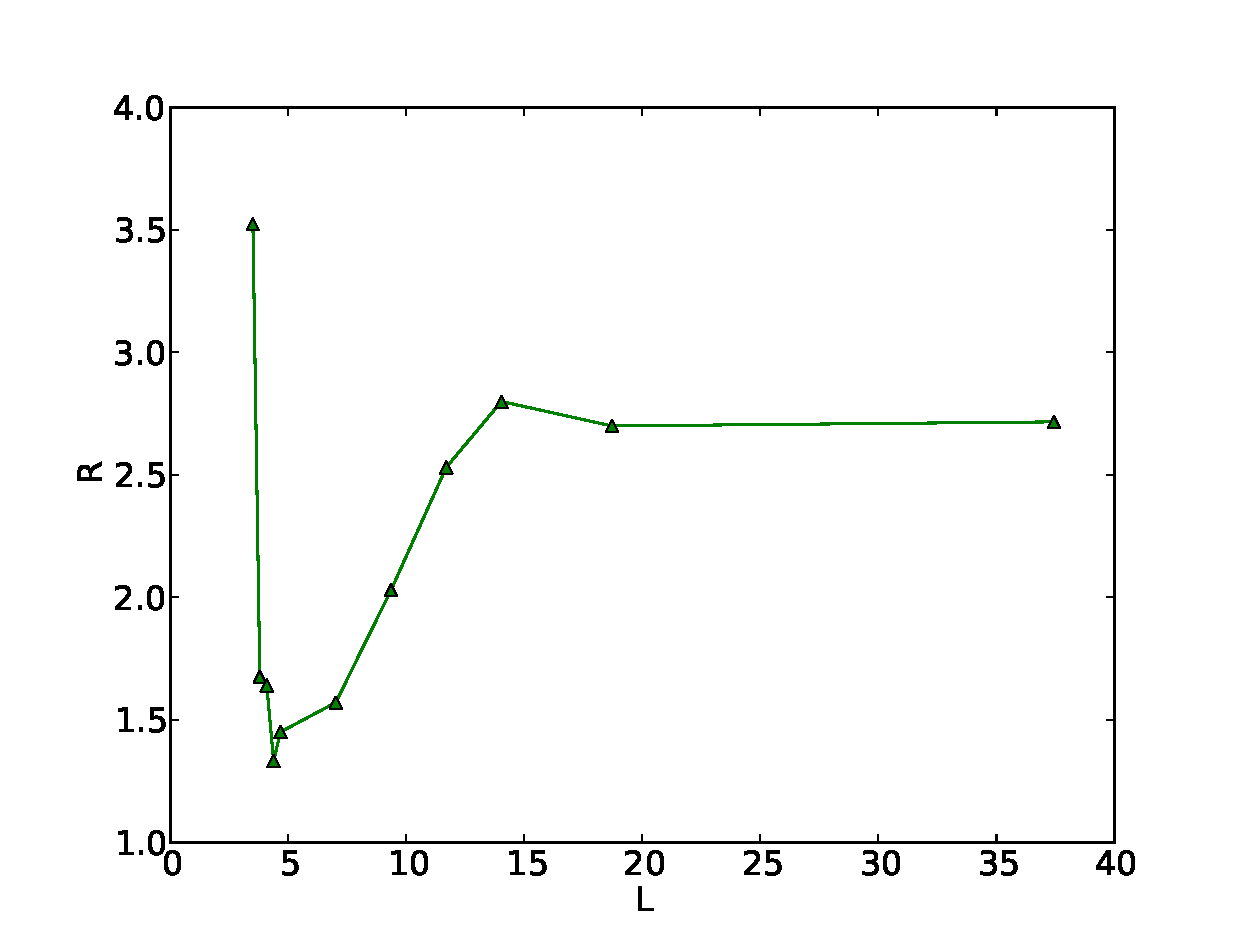
\includegraphics[width=0.45\hsize]{rc_vs_l.eps}
(b)
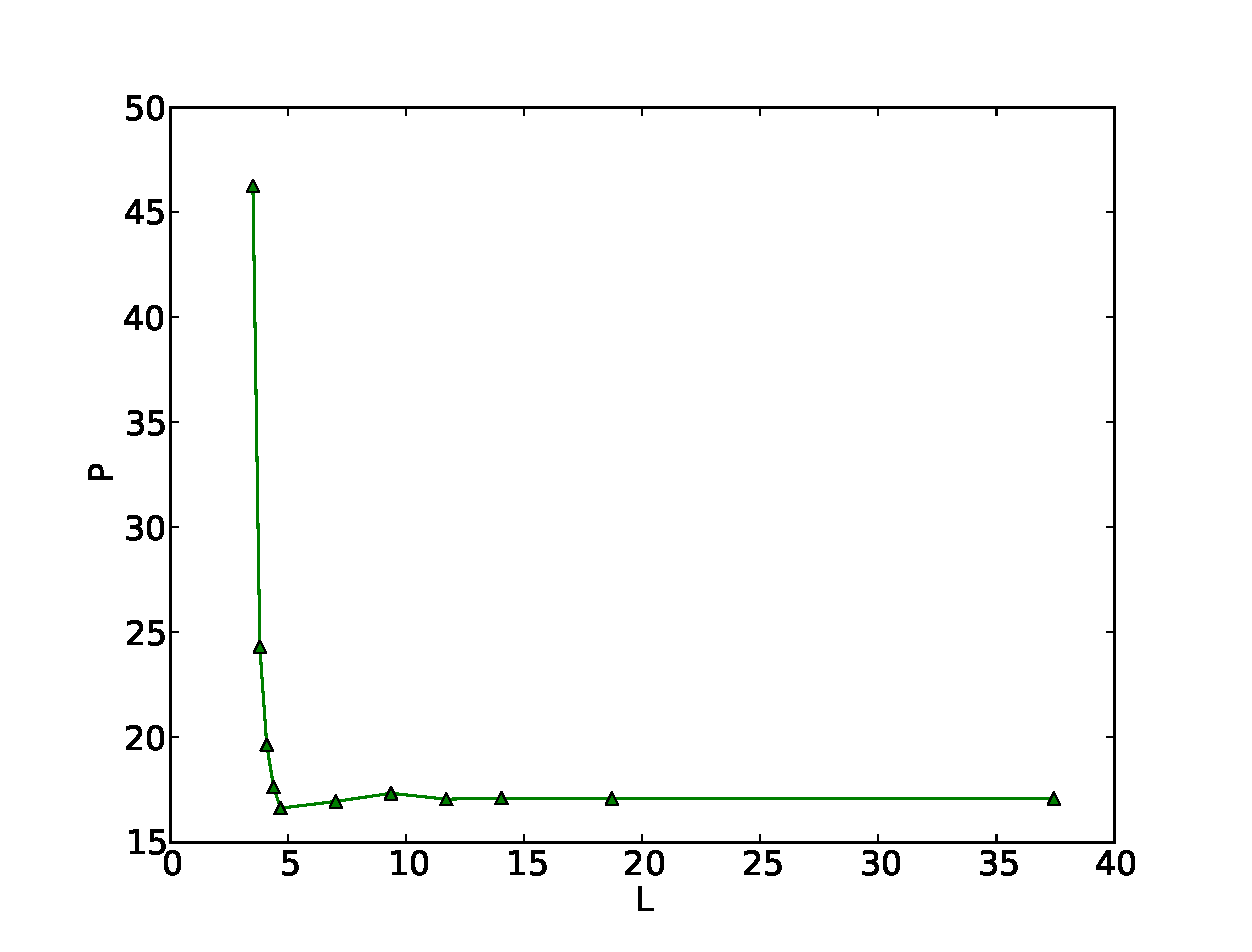
\includegraphics[width=0.45\hsize]{period_vs_l.eps}
\caption{ 
(a)
The rescaled radius of curvature measured at the middle link of a chain  versus the rescaled chain length in steady state for $h=0$.
(b)
The rescaled period  versus the rescaled chain length in steady state for $h=0$.
}
\label{fig:RvsL}
\end{center}
\end{figure}


Note that in Fig. \ref{fig:RvsL}(b) the period diverges for finite $L \approx 3$. Below this
point, the solution is a static straight line. This is similar to the usual buckling transition
for a finite length elastic rod. The microtubule needs to be sufficiently long to undergo
the dynamical instability analyzed here. 


\subsection{Selection of Scale}

As noted in section \ref{subsec:ScaleInvariance}, there exists
a continuous family of steady state solutions because  if
$\bw(\xi)$ is a solution, then so is $\bw(\lambda \xi)$ for arbitrary
$\lambda$. The general way that a particular value of $\lambda$ is selected
is likely to be due to the same mechanism as in other pattern formation
problems~\cite{Kessler,Barbieri}. The travelling wave solutions ignore the
boundary conditions at the ends $s=0$ and $s=L$.  Far from those ends,
we have found a continuous family of solutions. However these solutions
become invalid close to the ends.  The travelling wave solutions are
only valid in the limit of $0 << s << L$. The full solution must match
to one of these travelling solutions in that region but will differ
greatly near the ends.

As an example, consider the circular solutions of
Sec. \ref{subsec:CircularOrbits} with $h = \alpha = v_s = 0$. There the
steady state solution is a rotating circle wrapped around on itself of
{\em arbitrary radius} $R$.  However near the end $s=0$, the solutions
goes into the circle's center. Similarly it deviates from a circle
at $s=L$.  In analogy with other pattern growth problems such as the
``Geometric Model"~\cite{Kessler},  where the mathematics have been analyzed
in detail, we expect that the boundary conditions imposed on the ends,
will only be satisfied for certain values of $R$. If there is more than
one allowed value of $R$, the value picked out will be the most stable of
these. In the Geometric Model the form of the equations is much simpler,
making it possible to understand the overall structure of the problem
more easily. In the present case, a precise understanding of the numerical
results will be the subject of future research.


%%%END MATH PAPAER
This analysis was extended to non-zero $v_s$ and as shown in the supplemental materials~\cite{SupplMat}, does not
appreciably change the estimate we will give below for microtubule wave parameters in fast streaming oocytes. 


When the microtubule is tethered to an impenetrable surface (in this case, the oocyte cortex) and the external cytoplasmic streaming velocity $v_s$
is parallel to that surface, the form of the solution changes considerably. Numerical results show that the microtubule becomes completely two dimensional,
lying close to the surface. For low enough $v_s$, travelling wave
solutions are close to prolate cycloids, meaning that the microtubule periodically loops back
on itself (see supplemental movie 2~\cite{SupplMovies}. This can be understood analytically. For sufficiently large $v_s$ it transitions to other states finally becoming 
two dimensional and looking close to a sinusoid (see supplemental movie 3~\cite{SupplMovies}. This is analyzed in detail in
the supplemental materials~\cite{SupplMat}.

We have not included hydrodynamic and steric interactions between
different microtubules except in the approximate way of giving rise to
a constant cytoplasmic streaming velocity. 
The complete many body interaction is analyzed in chapter \ref{chap:Interact}, and we find that the microtubules do indeed have a strong tenndancy to self correlate into a single directed global flow. 
The wave like motion that we find is quite robust. Attaching microtubules together or
considering additional forces still leads to periodic or sometimes chaotic
motion, still at the same characteristic time and spatial scales. Therefore
despite the simplicity of the model, we expect that the basic length
and time scales that we predict should be quite robust.

\section{Comparison with Experiment and Discussion}

We now check to see whether the above model is consistent with experimental
results.  
Estimates of the microtubule elastic constant $C$ vary
considerably~\cite{Felgner,GittesRigidity}  but range mostly within 
$2$ to $4 \times 10^{-23} N m^2$. We estimate the force due to the kinesin
per unit length, $f_k$ to be its velocity $v_k$ times the cytoplasmic
viscosity. We will assume as suggested by our above analysis, that
$a/d$ is between $1/4$ and $1$. We will take the kinesin velocity $v_k$ to be approximately $1
\mu m/s$~\cite{SvobodaBlock,MeyhoferHoward}. The effective viscosity of the cytoplasm for small
particles has been studied extensively and appears to vary depending on the type of cell and on the length scale~\cite{LubyPhelps}. 
Particles of different sizes diffusing in the cytoplasm diffuse as if the medium had a different viscosity. Its viscoelastic properties will depend on many
factors such as the state of gelation of actin filaments~\cite{YinStossel}.
We will assume that during fast cytoplasmic streaming, the cytoplasmic actin is mainly in a "sol" state allowing fast streaming
to more readily take place. If this is not the case, the effective viscosity could be much higher~\cite{LubyPhelps}
but the dissipation would increase proportionally requiring a higher energy input. 
For small particles of radius approximately $20 nm$, the effective  viscosity 
as measured by diffusion is approximately 8 times that of water~\cite{LubyPhelps} and we will use this
value for comparison with experiment.  
This gives $f_k = (a/d) v \eta$ in the range  $2$ to $8 \times 10^{-9} N/m$.
Plugging these numbers into Eq. \ref{eq:R} gives $R$ in the range  $30$ to $50 \mu m$.
We can estimate the angular velocity using Eq. \ref{eq:Romega} (which
ignores cytoplasmic streaming). To get the largest range of times, we assume that the hydrodynamic drag
coefficient is due solely to the impellers, so that $\nu = (a/d) \eta$. This
is equivalent to $\omega = v_k/R$ or a period of $ T = 2 \pi R/v_k$ which ranges 
from $190$ to $310 s$.

Serbus and colleagues have observed microtubule behavior in living \emph{Drosophila} oocytes using GFP-tubulin 
and confocal fluorescence microscopy~\cite{SerbusSaxton}. 
Time-lapse movies showed bright fibrous fluorescence, representing
groups of microtubules, in a background of diffuse fluorescence from non-polymerized GFP-tubulin.
The microtubule patterns changed over time, as did the patterns of motion of organelles that
either excluded the GFP-tubulin or were themselves auto-fluorescent. Bends in the microtubules were
at times visible in the $x-y$ optical plane and some remained visible within that plane for $30-90 s$,
allowing measurement of a radius of curvature that we expect to approximately correspond to the
$R$ in the above analysis. $R$ was measured  to be $19.5\pm 6.5 \mu m$ with $9$ measurements (standard error $2.1 \mu m$),  and
the wave velocity was $v = 0.265 \pm 0.04 \mu m/s$ with $4$ measurements. Because these waves
appear roughly sinusoidal, we can also estimate the period $T$. Assuming a wavelength of $4R$
then the measured velocity gives a period of $T= 294 s$ with an even larger error bar
considering the fact that this assumes a waveform that is probably not accurate. Nevertheless
it suggests a characteristic time.



% The motion studied here can be contrasted with ciliary
% motion~\cite{Kennedy} which has a period on the order of $.05 s$. Clearly
% the two mechanisms have fundamentally different explanations. 
% The experimental time scale points to the mechanism described here rather
% than ciliary motion.  
The agreement found with experiment in our above
analysis is to some extent fortuitous, given the large uncertainties
in the experimental system. But nevertheless, it provides evidence that
the simple mechanism proposed is the origin of the behavior seen in
cytoplasmic streaming.  The experimental evidence~\cite{SerbusSaxton} that dynein inhibits
streaming and that minus ends of microtubules are in contact with the
cortex~\cite{ChaSerbus}, both support this hypothesis as well. 

More generally, the above analysis elucidates, at a qualitative level, the phenomena seen
in experiment~\cite{SerbusSaxton}, of strong cytoplasmic streaming
occurring concomitantly with wave-like motion of microtubules.
The movement of a relatively few number of kinesin motors on a microtubule 
couples to the fluid causing a bulk hydrodynamic flow. The force a
kinesin exerts on a microtubule sets the microtubule into motion causing
it to execute wave-like motion. This in turn causes the flow lines around microtubules to be time dependent,
making the microtubules act as stirrers for the surrounding fluid, which leads to 
chaotic flows and strong mixing~\cite{Aref,Aref2000}. 



\begin{figure}[htp]
\begin{center}
(a) 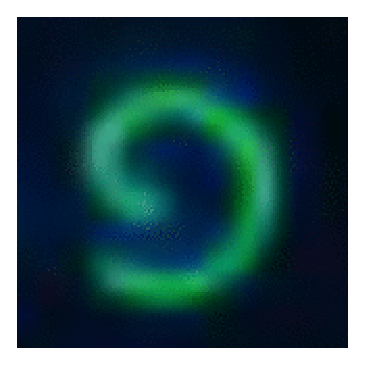
\includegraphics[width=0.3\hsize]{koch2.eps}
(b)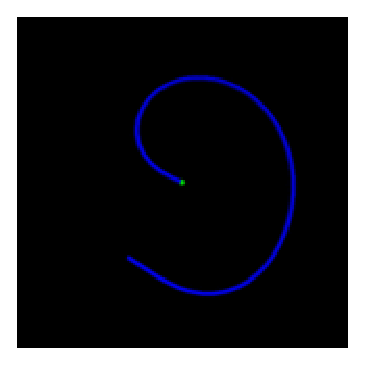
\includegraphics[width=0.3\hsize]{squiggle_sim.eps}
\caption{ 
The configuration a rotating microtubule in a gliding assay~\cite{MaloneyHerskowitzKoch,MaloneyKochVideo} with the leading end
stuck to a kinesin protein is shown in (a). (b) Shows the two dimensional simulation
of Eq. \ref{eq:microtubule} showing a similar shape.
}
\label{fig:squiggle}
\end{center}
\end{figure}


Can such motion be directly observed in an {\em in vitro}
experiment?  In fact it has been seen frequently as an unwanted artifact
of sample preparation.
Microtubule gliding assays were pioneered more than two
decades ago~\cite{ValeSchnappEtAl} and have become a
standard technique to better understand the motion of kinesin motors.
When a solution microtubules and ATP is placed on a glass surface on
which there is a high density of kinesin molecules, the kinesins propel
the microtubules with their minus ends leading.  Occasionally the minus
end sticks, perhaps to damaged kinesins, and continued forces of the
trailing portion of the microtubule cause flexing and curve generation.

Microtubule gliding assay videos of high quality~\cite{MaloneyHerskowitzKoch} provide an excellent
source of data for investigating the two dimensional version of the problem
studied here~\cite{MaloneyKochVideo}. The microtubule is being pushed by kinesin molecules
that on average, apply a force tangent to the microtubule. When an
end is tethered by sticking to a kinesin molecule, as noted above, this leads to 
a physical situation that is well described by Eq. \ref{eq:microtubule}. It should be
emphasized that the values of the tangential force $f_k$ and the drag
coefficient $\nu$ will be much larger than in the oocyte case.
Consequently, sometimes microtubules flex,, 
forming a G-shaped curve that rotates around the anchored minus end 
of the microtubule.  Fig. \ref{fig:squiggle} shows a comparison of
snapshots of the microtubule with that of a
simulation of Eq. \ref{eq:microtubule}. The resemblance is quite striking and provides evidence that
the theoretical modeling of this bending instability is valid. Note that
the shape obtained is independent of the values of model parameters. From
measuring the radius $R$ of the G-like configuration and its angular
velocity of rotation, we can compute both $f_k$ and $\nu$ from Eqs.
\ref{eq:R} and \ref{eq:Romega}, giving  $\nu = \omega C/(\beta R^4)$
and $f_k = \nu R \omega$. Measurements give $R \approx 1.33 \pm 0.2
\mu m$ and the period $T = 12 \pm 1 s$. Therefore $\nu = 133 N s/m^2$
and $f_k =  9.3\times 10^{-5} N/m$, both estimates are accurate within
a factor of 2 assuming that $C$ has been well determined.  The force
exerted by a kinesin motor in this situation is close to the experimentally determined stall
value of approximately $f_m = 5 pN$~\cite{MeyhoferHoward}. Assuming that
each motor attached can exert this force, this gives
an average distance between motors of $f_m/f_k = 53 nm$. This assumes that
the attachment of the motors is flexible enough to allow microtubule interactions capable of exerting this stall force. If
this is not the case, we expect the kinesins to be spaced more closely but
by no more than half this amount. This distance
seems reasonable given the high density of kinesin molecules attached
to the glass, and the size of the $\alpha-\beta$ tubulin dimer which is
approximately $8 nm$ in length. Thus the above considerations can give
a quantitative measure of the forces and drag in these gliding assays.


Nevertheless, it would also be of interest to verify the travelling wave solutions experimentally
in three dimensions for isolated
microtubules and kinesin, for example, by utilizing a single molecule optical trap, or by some other
means, allowing for a more rigorous test of the predictions made here.


It is of interest to speculate on the reason for this microscopic mixing
mechanism.  If the microtubules were attached from the {\em plus} end,
there would be no dynamical instability from kinesin generated forces
but the cytoplasmic streaming would be more efficient, with greater transfer
of force from outside the oocyte, because the tension at the
tether point would increase linearly with the length of the microtubule,
whereas the tension saturates to a constant value in the case considered
above. However as discussed earlier, complex stirring patterns are
expected to be far more efficacious in mixing than steady-state flows.
This agitation could then serve an important biological function.


In summary, we have found a very simple set of conditions for generating efficient mixing
in large eukaryotic cells. If microtubules are aligned so that their minus ends
are in contact with the cell perimeter and dynein is suppressed, this will lead 
(a) to cytoplasmic streaming in the bulk of the cell and (b) wave-like motion of
microtubules. The latter will promote efficient mixing of the cell's contents by
inducing chaotic flows.
The efficiency of the cytoplasmic streaming is due to the long range nature of
hydrodynamic coupling and the indirect linkage of microtubules to the oocyte surroundings via the cortex, leading to momentum transfer.
The wave-like motion is due to an instability in the dynamics which breaks chiral
symmetry and is a consequence of the tangential forces exerted by motor proteins on the elastic
microtubules. Given the uncertainties in the experimental system and approximations
made in the analysis, The wave-like motion seen in experiments agrees well with our theoretical predictions
suggesting these effects represent a robust phenomenon.
We are now engaged in experimentation to gather more accurate data on microtubule behavior 
{\em in vivo} and {\em in vitro} under various conditions in order to further understand
the mechanisms for fast cytoplasmic streaming discussed here.

% The authors would like to thank Ian Carbone, and Bill Sullivan for useful discussions.
% We also would like to gratefully acknowledge Andy Maloney and Steven J. Koch for their permission
% to use a snapshot of their video, Fig.  \ref{fig:squiggle}(a) \cite{MaloneyKochVideo} of their
% experimental results~\cite{MaloneyHerskowitzKoch}. This was generously distributed to us
% by them~\cite{KochLab} through the practice of Open Notebook Science~\cite{OpenNotebookScience} 
% This material is based upon work supported by National Institutes of Health GM046295 (to W.M.S.), National Science Foundation
% CCLI Grant DUE-0942207 (to J.M.D.),
% the  Defense Threat Reduction Agency basic research grant HDTRA-1-09-1-0018 (to Steven J. Koch),
% and the National Science Foundation IGERT Grant DGE-0549500 (to Steven J. Koch).




\section{Conclusions}

We have analyzed a model that describes a microtubule tethered at its minus
end and subject to viscous drag and forces due to kinesin walking toward the plus end. The walkers
provide a force tangent to the local direction of the microtubule and
cause an instability that causes nonlinear waves to travel along its
arclength. The scale of the wave can be arbitrary. An open question now 
is to find an analytic model that predicts the precise scale that
is selected. There are many other questions that are interesting.
What is the motion when there are obstacles that prevent free motion
of the microtubule? Do these lead to chaotic behavior? What happens
in the case of many microtubules interacting through steric and hydrodynamic
interactions? This last question is difficult to answer and is the subject of \ref{chap:Interact}. Velocity
flows giving rise to micro-mixing have been studied in related systems~\cite{GoldsteinTuvalvandeMeentPNAS,GoldsteinTuvalvandeMeentPRL,MeentSedermanGladdenGoldstein,VerchotLubiczGoldstein} and it would be very interesting to
understand the large scale cytoplasmic motion for \emph{Drosophila} oocytes.


%\section{Acknowledgements}

%The authors would like to thank Ian Carbone, and Bill Sullivan for useful discussions.
%5This material is based upon work supported by National Institutes of Health GM046295 (to W.M.S.), and National Science Foundation
%CCLI Grant DUE-0942207 (to J.M.D.).




%Multi poly stuff
\chapter{Fluid Mediated Polymer Interactions}
\label{chap:Interact}
Having studied the dynamics of individual polymers in an externally imposed flow field, we must now investigate how such a field could be brought about due to a large group of microtubules. 
In order to produce a global flow field in the fluid, we need a large number of microtubules all aligned and contributing to the driving of the field in a correlated manner. 
In addition to investigating steady state values, the behavior at low field could determine criteria under which spontaneous global velocity field formation could occur. In order to do these types of calculations, a more detailed view of the interaction between elements in the system needs to be taken.

\section{Introduction to the Oseen Tensor}
Since we are in a low Reynolds number regime, the motion of the fluid is described by the simplified Stokes equations:
\begin{equation}
\begin{array}{l}
\nabla p = \mu \nabla^2 \mathbf{u} +  \mathbf{f} \\
\nabla \cdot  \mathbf{u} = 0
\end{array}
\end{equation}
The linearity of the Stokes equations allows for solutions to be obtained via a Green's Function, such that for a continuous force density $ \mathbf{f}( \mathbf{r})$,
\begin{equation}
\label{eq:fluidgreensfunc}
\begin{array}{rcl}
 \mathbf{u}(\br ) &=& \int  \mathbf{f}(\br^\prime) \cdot  \mathbf{J} (\br - \br^\prime) d\br^\prime \\
p(\br) &=& \frac{ \mathbf{f}(\br^\prime) \cdot (\br - \br^\prime)}{4 \pi | \br - \br^\prime|^3} d\br^\prime
\end{array}
\end{equation}
Where 
\begin{equation}
\label{eq:oseentensordef}
 \mathbf{J}(\br) = \frac{1}{8\pi\mu} \left( \frac{I}{|\br|} + \frac{\br\br^T}{|\br^3|}\right)
\end{equation}

is a second rank tensor field known as the Oseen Tensor.
The Oseen tensor has had great success in describing how small or thin objects interact in fluid, as well as the self interaction of polymers. 
In general the Oseen tensor has higher order corrections in $a/R$, but these begin at $(a/R)^3$ and should not play a significant role in cross polymer interactions.
Of particular interest is its use in modeling polymers as a long chain of beads, which will lend itself well to numerical simulation.
%[***Cite some places using the tensor***]

\section{Model for Hydrodynamic Interactions}
For our model, we are going to use the same structure for the microtubule as for the solitary case. This models the microtubule as a chain of beads with some tension $T$ and stiffness parameter $C$. The equation of motion for the microtubule is very similar, except now we need to include the Oseen interaction tensor.
The microtubule and impellers are in direct contact with the fluid and at the interface the velocity of the fluid must match the velocity of the objects suspended in it.
This means that any force exerted on the objects will also be transmitted to the fluid locally. 
These forces form the force density used in the Oseen tensor to determine the fluid velocity in all of space, which will also determine the motion of the microtubule impeller system.

This is a bit more complex than simply adding the tensor to the previous equation of motion, as the interaction tensor needs to include the forces of all objects moving in the fluid. 
Before we simply included the kinesin as a force tangent to the backbone of the microtubule, and while that is still going to be our model, we now need to include consideration for the reaction force produced against the impeller, as this will be transmitted back to the microtubule by the long range hydrodynamic forces.
In order to determine the effect that this extra force density will have on the dynamics, we need to be more explicit with the configuration of the impellers.
Consider the impellers of largest dimension $q$ to be attached to the microtubule by kinesin motors with no side being preferred at a characteristic distance $a$ with, as in the single microtubule consideration, $a < q \ll L$, with $L$ again being the microtubule length. 
We can consider this to form a uniform density of impellers around the microtubule, and the kinesin motors cause the impeller and the microtubule to move relative to each other with a fixed velocity in the direction of the tangent of the microtubule backbone. 
\begin{figure}[htp]
\begin{center}
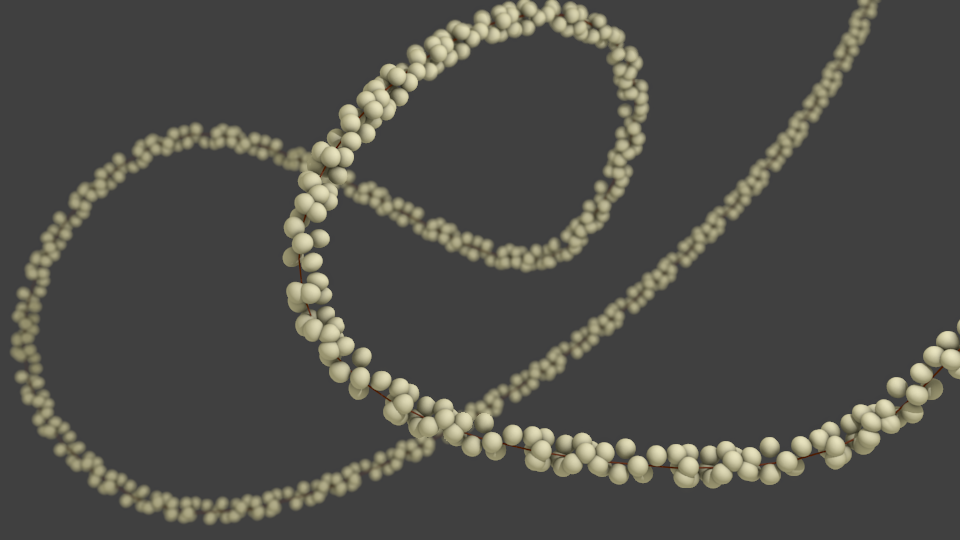
\includegraphics[width=\hsize]{impeller.png}
\caption{ 
The impellers are carried along the microtubule by the kinesin motors. Kinesin is a small protein, so the impellers are arranged very close to the microtubule relative to the impeller size as well as the characteristic buckling length of the microtubule, which is itself very thin.
}
\label{fig:impellerpic}
\end{center}
\end{figure}
\begin{equation}
\label{eq:fluidmodel}
 \mathbf{u}(\br) =  \int \left[ \mathbf{J}(\br-\br^\prime(s))[-C \frac{\partial^4 \br^\prime}{\partial s^4} + \frac{\partial}{\partial s}(T(s)\frac{\partial \br^\prime}{\partial s}) - f_k \frac{\partial \br^\prime}{\partial s}] + \int  \mathbf{J}(\br-\br^\prime(s)+ \mathbf{a}(s)) \frac{ \mathbf{f_k}}{2\pi| \mathbf{a}|} \frac{\partial \br^\prime}{\partial s} d \hat{ \mathbf{a}} \right] \;ds
\end{equation}
where $ \mathbf{u}$ is the fluid velocity and $ \mathbf{a}$ is a vector pointing radially outward from the microtubule axis to the impeller location. 
Because the microtubule system is in contact with the fluid, the motion of the microtubule will follow that of the fluid along the backbone locations.
However, due to the long range of the hydrodynamic interaction, the system can now be far more sensitive to the overall configuration which could potentially lead to more complex steady state solutions than the non interacting single microtubule.

%%%force diagrams

\begin{figure}[htp]
\begin{center}
(a)
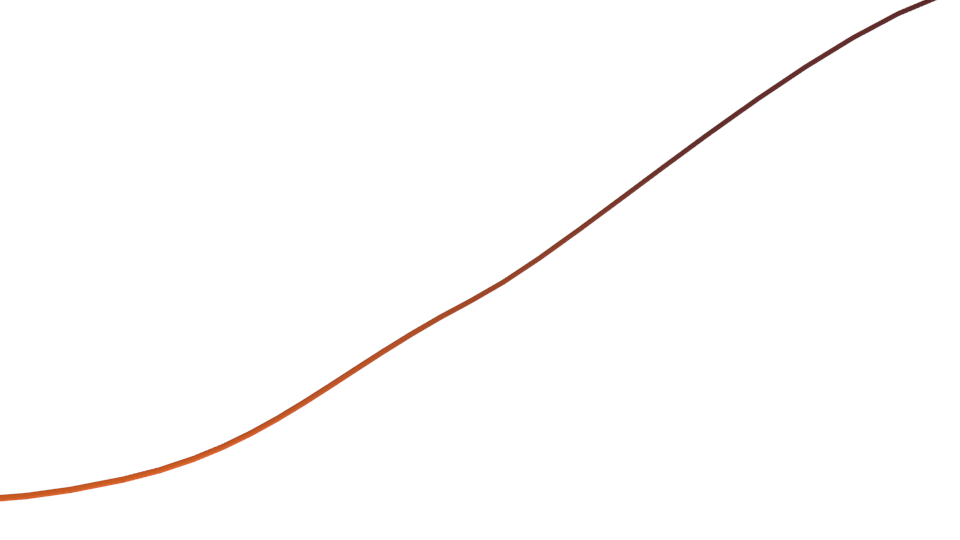
\includegraphics[width=0.45\hsize]{gradforces.png}
(b)
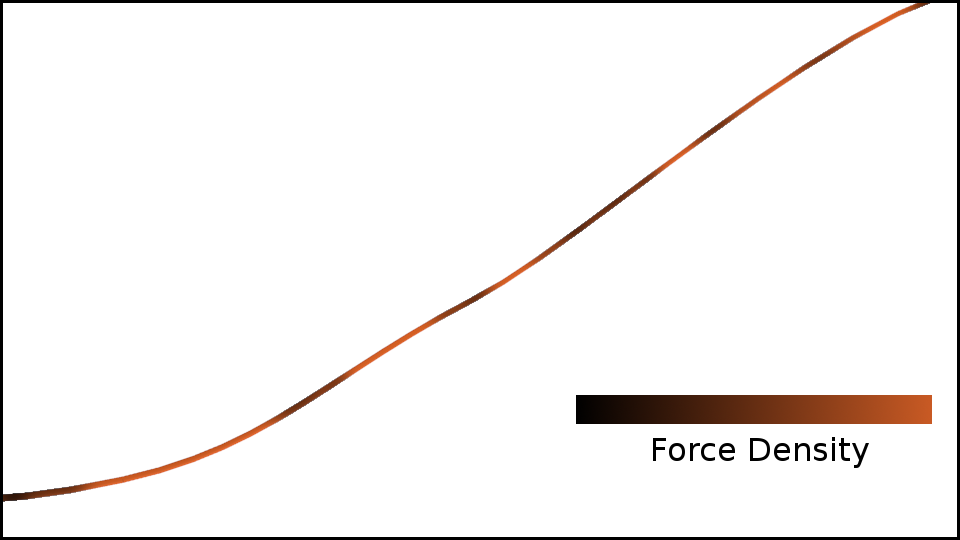
\includegraphics[width=0.45\hsize]{stiffforces2.png}
(c)
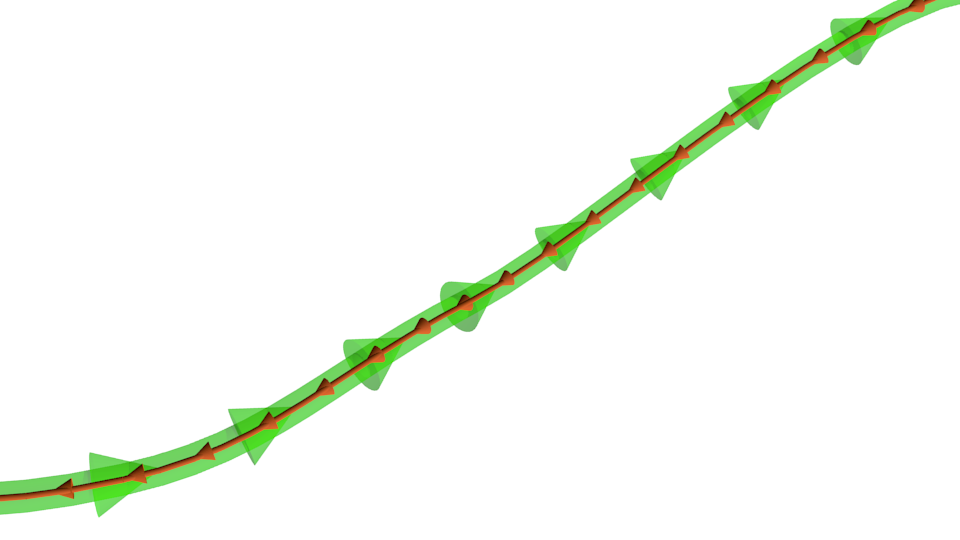
\includegraphics[width=0.45\hsize]{ktforces.png}
\caption{ 
(a)
A gradient in tension creates a force density along the axis of the microtubule backbone. This is determined by the microtubule configuration.
(b)
The microtubule curvature creates a force density that acts on the fluid. This is also determined by the microtubule configuration.
(c)
The kinesin motors act on both the microtubule and the impellers, applying forces that bind them together and drive the impellers along the microtubule. Both of these force densities are transmitted to the fluid. These force densities arise due to a local coupling. and therefore are related by Newton's third law.
}
\label{fig:forcedensities}
\end{center}
\end{figure}

There are three primary generators of force; backbone stiffness, a gradient in backbone tension, and the kinesin motors. The first two force densities can be computed entirely from the microtubule configuration, and these values can then be used as inputs to the Oseen tensor.
The force due to the kinesin coupling and walking is much harder to work out, however, we will show that it has negligible effect on the long range fluid motion.

%thus begins the math to show its a quadrapole
\subsection{Kinesin Quadrapole}
In order for the kinesin to drag the impeller along, it must pull against the microtubule, and as such the force dragging the impeller through the fluid has a corresponding opposite force on the microtubule by Newton's third law. 
Both of these forces are then transmitted to the fluid, so it seems reasonable to try to express these forces as some multipole expansion in a small parameter.
The microtubules have a significant stiffness which leads to a characteristic buckling length as described in Eq. \ref{eq:R}, which sets a size scale for features of the microtubule motion. Compared to this size scale, the impellers are very small, and bound very tightly to the microtubule backbone. 
In addition to this, we are assuming that the impellers are attached to the microtubule in a cylindrically symmetric fashion. This leads to a small scale force distribution that looks like a classic quadrapole configuration, as shown in figure \ref{fig:quadforce}.

\begin{figure}[htp]
\begin{center}
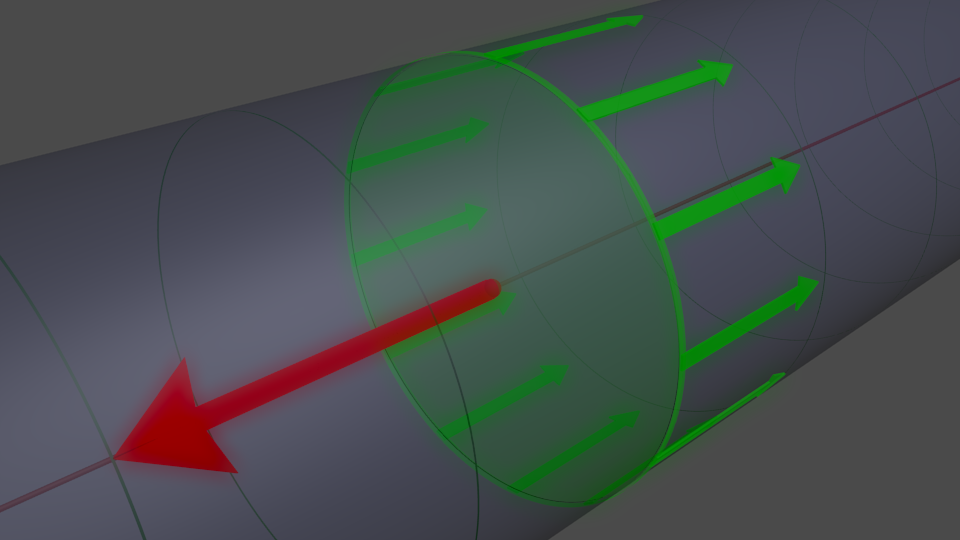
\includegraphics[width=\hsize]{segforce.png}
\caption{ 
At a given location along the microtubule, the forces generated by the kinesin motors push between the microtubule and the impellers. This force density has a cylindrically symmetric shape, which contributes to a rapid falloff in the effect it has on the fluid.
}
\label{fig:quadforce}
\end{center}
\end{figure}

Let us investigate the contribution to the fluid velocity field from a small segment of the microtubule impeller system. For convenience, place the segment at the origin, and calculate the fluid motion at position $\br$. The kinesin motors apply force between the microtubule and impellers in two ways. They walk along the axis of the microtubule producing the significant force along the axis, and they also hold the impellers onto the microtubule, creating a rigid link force radially. A key feature of the nature of these forces is symmetry of inversion through the center axis.

We can now write down the fluid response due to this force density.
\begin{equation}
\label{eq:forcedensitystart}
\delta \mathbf{u}(\br) = \frac{1}{8\pi\mu}\int \frac{ \mathbf{f}}{|\br +  \mathbf{a}|} + \frac{(\br+ \mathbf{a}) ((\br +  \mathbf{a}) \cdot  \mathbf{f})}{|\br +  \mathbf{a}|^3} d\hat{ \mathbf{a}} - \frac{ \mathbf{F}}{|\br|} - \frac{\br (\br \cdot  \mathbf{F})}{|\br|^3}
\end{equation}
Where $\delta  \mathbf{u}(\br)$ is the contribution to the fluid velocity at position $\br$ from a differential segment of the microtubule impeller system, $a$ is the vector pointing from the center of the microtubule to a point in the impeller sheath, $F$ is the linear force density on the microtubule backbone produced by the kinesin walkers, and $f$ is an area force density of the force needed to drag the impeller sheath through the fluid. 
Because the kinesin binds the microtubule and the impeller together, Newton's Third Law dictates that the linear force density along the backbone needs to be equal and opposite for the impeller microtubule pair. This gives us that integrating $f$ around the full circle must give the same value as $F$.
Due to the small size of the kinesin molecule, for long range interaction on the order of the length of the microtubule, or even characteristic curvatures of the microtubule, we should have $a << r$, where $a$ and $r$ are the magnitudes of $ \mathbf{a}$ and $\br$ respectively. We can pull out a factor of $r$ to obtain these expressions in terms of a unit-less small parameter $\epsilon = a/r$.
\begin{equation}
\label{eq:forcedensitycircleonly}
\int \frac{ \mathbf{f}}{|\br +  \mathbf{a}|} + \frac{\br (\br \cdot  \mathbf{f})}{|\br +  \mathbf{a}|^3} d \mathbf{a}
\end{equation}
%bad form?
Becomes
\begin{equation}
\label{eq:forcedensityepsilon}
\int \frac{\bf f}{r|\hat{\br} + \epsilon \hat{ \mathbf{a}}|} + \frac{(\hat{\br} + \epsilon \hat{ \mathbf{a}}) ((\hat{\br} + \epsilon \hat{ \mathbf{a}}) \cdot  \mathbf{f})}{r|(\hat{\br} + \epsilon \hat{ \mathbf{a}})|^3} d\hat{ \mathbf{a}}
\end{equation}
Apart from a global factor of $1/r$, only the directions of $\br$ and $ \mathbf{a}$ remain, with all of the distance scaling being absorbed into the small parameter $\epsilon$. We can now expand the expression to find what the leading order contribution to the fluid velocity field will be.
The zeroeth order term reduces simply to
\begin{equation}
\label{eq:forcedensityzeroth}
\delta \mathbf{u_0}(\br) = \int \frac{\bf f}{r|\hat{\br}|} + \frac{(\hat{\br}) (\hat{\br} \cdot \mathbf{f})}{r|(\hat{\br})|^3} d\hat{\ba} - \frac{\bf F}{|\br|} - \frac{\br (\br \cdot \bf F)}{|\br|^3}
\end{equation}
Which will vanish due to the requirement of Newton's Third Law.
The first order term in $\epsilon$ requires a bit more work, but is still a straight forward derivative. We first need to expand the magnitudes in terms of a square root, and then proceed as normal.
\begin{equation}
\label{eq:forcedensityfirst}
\delta \mathbf{u}(\br) = \frac{1}{r} \int  \mathbf{f}[(\hat{\br} + \epsilon\hat{\ba})^2]^{-1/2} d\hat{\ba} +(\hat{\br} + \epsilon\hat{\ba})(\hat{\br} + \epsilon\hat{\ba})\cdot \mathbf{f} [(\hat{\br} + \epsilon\hat{\ba})^2]^{-3/2} d\ba - \frac{\bf F}{|\br|} - \frac{\br (\br \cdot \mathbf{F})}{|\br|^3}
\end{equation}

\begin{equation}
\begin{array}{rcl}
\label{eq:forcedensityfirstderiv}
\frac{d}{d\epsilon} \delta \mathbf{u}(\br) &=& \frac{1}{r} \int 
-\mathbf{f} [(\hat{\br} + \epsilon\hat{\ba})^2]^{-3/2} (\hat{\br} + \epsilon\hat{\ba})\cdot \hat{\ba} \\
&+&\hat{\ba}(\hat{\br} + \epsilon\hat{\ba})\cdot \mathbf{f} [(\hat{\br} + \epsilon\hat{\ba})^2]^{-3/2} \\
&+& (\hat{\br} + \epsilon\hat{\ba})(\hat{\ba}\cdot\mathbf{f})[(\hat{\br} + \epsilon\hat{\ba})^2]^{-3/2}\\
&-& 3 ((\hat{\br} + \epsilon\hat{\ba})(\hat{\br} + \epsilon\hat{\ba})\cdot\mathbf{f} [(\hat{\br} + \epsilon\hat{\ba})^2]^{-5/2} (\hat{\br} + \epsilon\hat{\ba})\cdot \hat{\ba}
\end{array}
\end{equation}
\begin{equation}
\begin{array}{rcl}
\label{eq:forcedensitylimit}
\lim_{\epsilon\to 0} \frac{d}{d\epsilon} \delta \mathbf{u}(\br) &=& \frac{1}{r} \int 
-\bf f [(\hat{\br})^2]^{-3/2} (\hat{\br})\cdot \hat{\ba} \\
&+&\hat{\ba}(\hat{\br})\cdot \mathbf{f} [(\hat{\br})^2]^{-3/2} \\
&+& (\hat{\br})(\hat{\ba}\cdot\mathbf{f})[(\hat{\br})^2]^{-3/2} \\
&-& 3 ((\hat{\br})(\hat{\br})\cdot\mathbf{f} [(\hat{\br})^2]^{-5/2} (\hat{\br})\cdot \hat{\ba}
\end{array}
\end{equation}

As we can see, each term in the integrand is an odd function of $\hat{a}$, and the integral is around the whole circle, so this vanishes. 
This means that the leading order term from the kinesin coupling force density is going to be suppressed by two factors of the small parameter $\epsilon$.
In comparison, the tension can be decomposed into equal and opposite pairs between adjacent segments of the microtubule. However, we will find that they are not able to form a quadrapole like the kinesin forces do.
\begin{figure}[htp]
\begin{center}
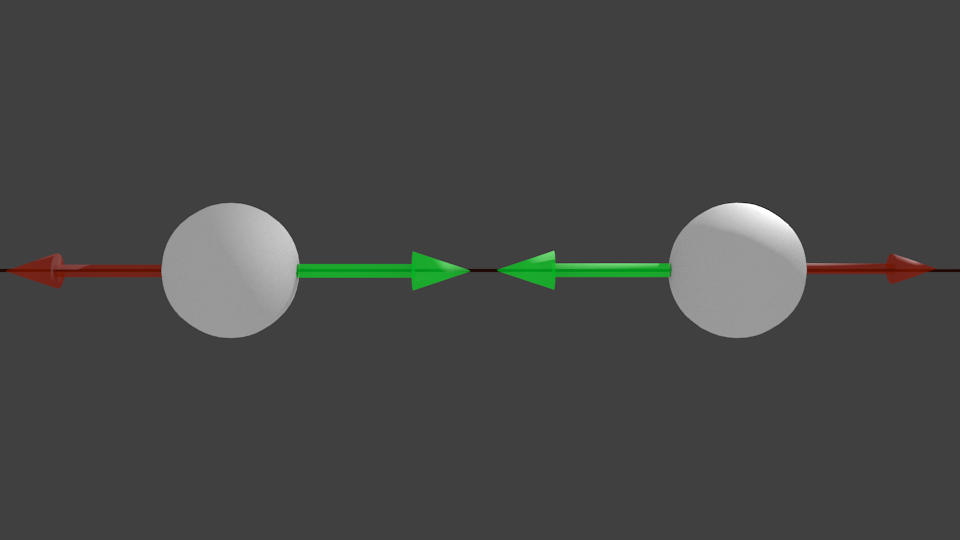
\includegraphics[width=\hsize]{tenbal.png}
\caption{ 
While the forces connecting the microtubule backbone must balance, these forces are a) axial and lack the symmetric cancellation of the quadrapole and b) the separation between them is the basis for the characteristic length scale of the microtubule itself, and is thus fixed in relation to the size scale of the interaction.
}
\label{fig:tenforce}
\end{center}
\end{figure}
The separation between the two opposing forces is axial, and lacks the mirror symmetry needed to form the quadrapole. This means that it would give rise to a dipolar term.
And even in the case of the dipolar term,  the corresponding small parameter needed to form the multipole cancellation is directly tied to the characteristic length scale of the microtubule curvature; indeed, the curvature is defined by these forces. 
So not only would it be a chain of dipoles, the density of those dipoles would need to diverge in the limit of small separation between the opposing forces.
Luckily, if we instead sum the forces on each individual segment, we are left with the simple linear force density of the gradient of the tension. This gradient is expected to be nonzero due to the tethering of one end of the microtubule.
A nonzero linear force density along the axis of the microtubule would apply directly through the Oseen tensor with no cancellation, and thus fall off as $\br^{-1}$, where as we saw the kinesin forces fall off as $\br^{-3}$.
 
That is not to say that the kinesin does not effect the system at all.

While the long range fluid motion will not be strongly influenced by the kinesin motor forces, these short range effects will allow the impellers and microtubule to move relative to each other. While the details of the local fluid motion are complex, the bulk effect is known; the kinesin walk along the microtubule at a steady rate, creating a fixed relationship between the impeller velocity and the microtubule velocity. 
Because the relative motion between the microtubule and the impeller layer is known, only the motion of the fluid at the impeller interface is needed to determine the motion of the system. 
As we have shown, the forces do to the kinesin motors directly do not contribute to the long range fluid motion, and the only remaining forces are those from microtubule backbone.

%describe fluid coupling
This leads us to a method for determining the dynamics of the system. The Oseen tensor should be integrated over the force densities $f_{int}$along the backbone of the microtubule, ignoring the contribution from the impeller directly. 
\begin{equation}
\label{eq:fluidvelocity}
\mathbf{u}(\br ) = \int_{backbone} \mathbf{f}_{int}(\br^\prime) \cdot \mathbf{J} (\br - \br^\prime) d\br^\prime
\end{equation}
This will give us the large scale fluid motion which will determine the large scale motion of the entire system. The coupling from the fluid back to the impeller microtubule system will depend on the short range fluid interactions brought about by the kinesin motors, however, we still expect the long range motion to match with the fluid. By symmetry, the difference in velocities will be axial, and the kinesin will still maintain a fixed relationship between the microtubule and impeller. From that we expect the fluid velocity to appear to be a weighted average of the microtubule and impeller velocity.
\begin{equation}
\label{eq:systemvelocity}
\mathbf{u}(\br) = \mathbf{v}_I(1-\delta) + \mathbf{v}_M \delta
\end{equation}
Where $\mathbf{v}_I$ and $\mathbf{v}_M$ are the impeller and microtubule velocities, respectively. If we use the relation between these two velocities we find an expression for our microtubule velocity
\begin{equation}
\label{eq:mtubevelocity}
\frac{d \br}{dt} = \mathbf{v}_M = \mathbf{u}(\br) - (1-\delta)v_k \frac{\partial \br}{\partial s}
\end{equation}
where $v_k$ is the kinesin walk speed. As we can see, the effect of the coupling on the microtubule motion is to suppress the kinesin walk speed by some fraction, just as in the single microtubule discussion. 
The geometry of the impeller microtubule arrangement, with the impellers forming a cylindrical sheath around the microtubule, suggests that the long range fluid motion would match more closely with the impeller velocity. This is added to by the fact that the characteristic size of the impeller is expected to be much greater than the microtubule thickness giving them more sensitivity to long range fluid motions.
This leads us to believe that $\delta$ should be a small number, and that the fluid couples almost entirely to the impellers.
Even if that is not the case, while the exact value of this suppression depends on the detailed interaction between the microtubule and impellers, the large scale behavior can be obtained by a simple rescaling of the walk speed, giving us the simple relation:
\begin{equation}
\label{eq:backbonevelocity}
\frac{d \br}{dt} = \mathbf{u}(\br ) - \mathbf{v}_k \frac{\partial \br}{\partial s}
\end{equation}

\section{Hydrodynamics near a hard wall}
Up until now, we have only considered microtubules pinned at one end freely floating in the cytoplasm, but in a biological system, the microtubules are believed to be anchored to the cell cortex. 
The presence of this stationary wall may have a significant effect on the microtubule motion, as it imposes a new boundary condition on the fluid motion; namely that the velocity must vanish at the cortex.

This new boundary condition changes the greens function used to construct the fluid velocity from the forces applied to the system. The determination of this greens function is dependent on the specific boundary geometry, and potentially intractable.
Because of this difficulty, we will first investigate the case of an infinite plane hard wall at $z=0$. Hopefully, this should provide some insight into the behavior of the microtubule impeller system near the cortex.

Fortunately, the Green's function for the infinite wall case has already been solved[***CITE***]. The technique is  similar to that of the method of image charges in classical electromagnetism, with the added complication of the sources being vector quantities instead of scalers. This vector nature of the sources gives rise to a number of corrections to the simple reflection.
Unfortunately, it is somewhat complex, though luckily not of higher order scaling than the unmodified Oseen tensor. The interaction $\mathbf{J}^w(\mathbf{x},\mathbf{y})$ between a point force $\bf f$ at location $\bf x$ and a fluid location $\bf y$ is now:
\begin{equation}
\label{eq:oseenwall}
\mathbf{J}^w(\mathbf{x}, \mathbf{y}) = \frac{1}{8\pi\mu \br^*} [ 
- (\mathbf{I} + \frac{(\br^*\cdot\mathbf{f})\br^*}{\br^{*2}}) 
+ \frac{2 h}{\br^{*2}}( (\frac{3 x_3(\br^*\cdot\tilde{\mathbf{f}})}{\br^{*2}} \br^* - \tilde{\mathbf{f}}_3)\br^* - x_3\tilde{\mathbf{f}} + (\br^*\cdot\tilde{\mathbf{f}})\hat{\mathbf{z}})]
\end{equation}
Where $\br^*$ is equal to $(x_1-y_1,x_2-y_2,x_3+y_3)$, the reflected displacement vector, $h = y_3$ the distance of the fluid from the wall, and $\tilde{\mathbf{f}} = (f_1,f_2,-f_3)$, the reflected force. 
One can recognize the first term as the reflected Oseen tensor, similar to a negative charge in the method of images. 
However, as previously mentioned, the fact the force must also have its direction flipped adds several additional terms. These terms together ensure that the velocity of the fluid will vanish at the boundary.

Other than the modification of the interaction tensor, the model remains almost unchanged.
Due to the assumptions used to generate this solution, it is of course only valid for $z>0$, and can result in very strange behaviors if applied for regions below the plane. 
These usually result in extremely singular velocities, and so extra care must be made to ensure that no part of the finite time step used in a simulation will cross this boundary. 
To ensure this, a hard wall potential similar to that used for the hard core repulsion of the microtubule segments is placed at $z=0$.

\section{Numeric Implementation of the Model}
The complexity of the interaction makes analytic solutions difficult, however, the dependence of the fluid flow only on the current state of the microtubule makes it suitable for direct simulation. A straightforward integration of the velocity field will yield the complete system dynamics.
\subsection{The discrete model}
As with the single microtubule case, the microtubules are modeled as a chain of discrete points. Unfortunately, the use of the long range fluid interactions prevents us from using pure rigid links, so this model uses a backbone comprised of stiff spring links, such that the force on each element is:
\begin{equation}
\label{eq:discretespring}
\mathbf{T}(\br_i) = k_T ( |\mathbf{d}_{i-}| - l )\hat{\mathbf{d}_{i-}} + ( |\mathbf{d}_{i+}| - l )\hat{\mathbf{d}_{i+}}
\end{equation}
With 
\begin{eqnarray*}
\mathbf{d}_{i-} &= \br_{i-1} - \br_i \\
\mathbf{d}_{i+} &= \br_{i+1} - \br_i
\end{eqnarray*}

Where $\br_i$ are the positions of the individual microtubule segments, with $k_T$ being the backbone spring constant and $l$ being the rest length of the segment. 
The spring constant is chosen to be as strong as possible for the given time step, in order to match as closely as possible to and incompressible chain.
In addition to the spring force tension term, the backbone stiffness is modeled as a discrete fourth derivative along the spine, with an adjustable scaling parameter.
\begin{equation}
\label{eq:discretestiff}
\mathbf{C}(\br_i) =  - k_C[ (\br_{i+2} - \br_i) - (\br_i - \br_{i-2})]
\end{equation}

In order for the microtubules to not cross through each other, they are also given a hardcore repulsion force that is divergent at zero distance along with rapidly and smoothly falling off to zero at some characteristic radius $d$.
This was implemented as a inverse fourth power law with a cutoff:
\begin{align}
\label{eq:discretehardcore}
\mathbf{h}(\br_i,\br_j) &= \begin{cases}(1 - \frac{d^4}{|\br_i - \br_j|^4})(\br_i - \br_j),&  \text{for } |\br_i - \br_j| < d \\
0,& \text{for } |\br_i - \br_j| \ge d \end{cases}\\
\mathbf{H}(\br_i) &= \sum_j \mathbf{h}(\br_i,\br_j)
\end{align}

In addition to the bulk forces, there are also boundary cases, as well as pinning the endpoints of the microtubule. The pinning is accomplished simply by including a spring force, similar to the tension spring force, that is centered to a specific fixed point in space.
All of these forces are directly transmitted to the fluid, and thus must be included in the Oseen tensor calculation. There is a difficulty when transitioning to the discrete case due to the singularity of the Oseen tensor at the origin. 
For this reason, the effect of the forces generated on a specific segment on the fluid at the same location is more difficult to determine.
%By symetry, one would expect that any effect on the fluid should share direction with that of the force generating it, and as such we can use the fact that the contribution to the fluid motion is proportional to the force to introduce an adjustable parameter to scale this effect. Because this is occurs locally, we don't expect this to effect the long range behavior of the system as a whole. 
The standard practice in this case is to use the Oseen tensor as an interaction between elements, and to use a simple free draining drag model for the local motion. Since our model is that of a long chain of beads we simply use the drag due to a small sphere.
\begin{equation}
\label{eq:discreteself}
\mathbf{J}_{ii} = \frac{1}{4\pi\mu}
\end{equation}
By combining equations \ref{eq:discretespring}, \ref{eq:discretehardcore}, \ref{eq:discretestiff}, and \ref{eq:fluidvelocity}, we see that for any point in space, the fluid velocity is given by:
\begin{equation}
\label{eq:discretesum}
\mathbf{u}(\br_i) = \mathbf{J}_{ii}[T(\br_i) + C(\br_i) + H(\br_i)] + \sum_{j\neq i} \mathbf{J}(r_i - r_j) [T(\br_j) + C(\br_j)+ H(\br_j)]
\end{equation}
However, due to the relative velocity between the fluid and the microtubule backbone, the velocity used to update the position of the microtubule locations $r_i$ is found by subtracting the kinesin walk speed.
\begin{equation}
\label{eq:discretevel}
\frac{d \br_i}{dt} = \bf u(\br_i) - \frac{1}{2}v_k (\br_{i-1} - \br_{i+1})
\end{equation}
This derivative is then used for a standard fourth order Runge Kutte integration in order to advance the system in time.

\section{Single Microtubule verification}
The new algorithm was then used to simulate a single microtubule in order to see what effect the fluid interaction would have on the single microtubule solution.
Because this simulation does not apply any external flow fields, we expect the solution to closely resemble the zero field case from the theory without fluid coupling.

We ran this simulation using the same parameters for a single microtububel with and without the fluid interaction, again using a random starting configuration and tethering the minus end of the microtubule to a fixed point in space. 
The result was essentially as expected, with a solution that asymptotically approached a circle rotating at a constant rate. A typical solution is shown here:

\begin{figure}[htp]
\begin{center}
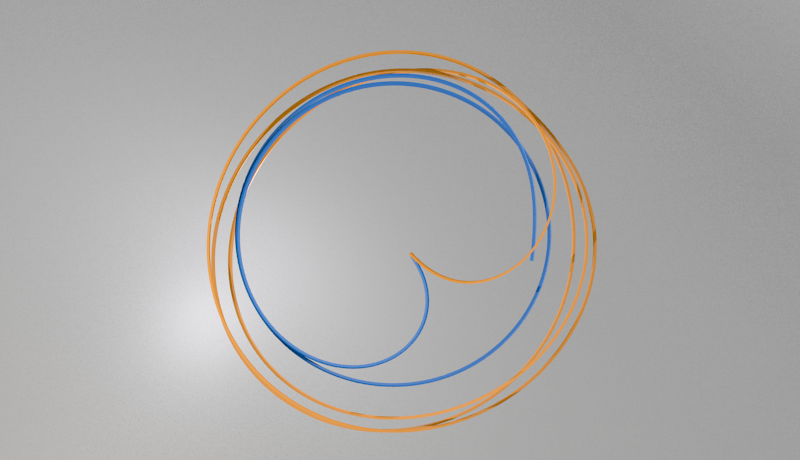
\includegraphics[width=\hsize]{singtest.png}
\caption{ 
Simulation results for a single polymer without fluid interaction(blue) and with fluid interaction(orange), with all other parameters held the same. They are qualitatively the same, though the radius is slightly larger with fluid interactions activated.
}
\label{fig:singtest}
\end{center}
\end{figure}

It is interesting to note that the hydrodynamic interaction have little to no effect on this type of solution. 


\section{Properties of the Many Polymer Model}

Now more microtubules are added to the simulation, so that there are on the order of tens to hundreds of them.
The microtubules have their minus ends anchored in a planar configuration, in order to closely resemble attachment to the cortex.
The spacing between the individual anchors can be varried, but will never be close enough for their hardcore radii to overlap.
This grouping of microtubules exhibits additional behaviors not found in the single microtubule system.

\subsection{Important Length Scales}
The introduction of more than one microtubule, along with the addition of the hard wall, introduce new length scales to the system.
The microtubules are placed with their anchor points in a plane. 
Within this plane, the anchors have a characteristic separation,$R_s$, and this separation defines one of the new length scales in the system.
The plane of anchors is parallel to the hard wall, but not directly on it. 
The separation between the hard wall and the plane of anchors, $h$ is a second new length scale.
These two new lengths are usually set to be less than the characteristic buckling length of the microtubule, $R_b$, in order to more closely match what is seen in the biological data.
We will see that these two length scales play an important role in determining the correlation behavior of the system.

\subsection{Correlation between multiple microtubules}
A key feature found during fast streaming in the biological system is the formation of correlated groups to enable larger scale coordinated forces on the fluid. 
These correlations can be seen in various experiments performed here [cite].

\begin{figure}[htp]
\begin{center}
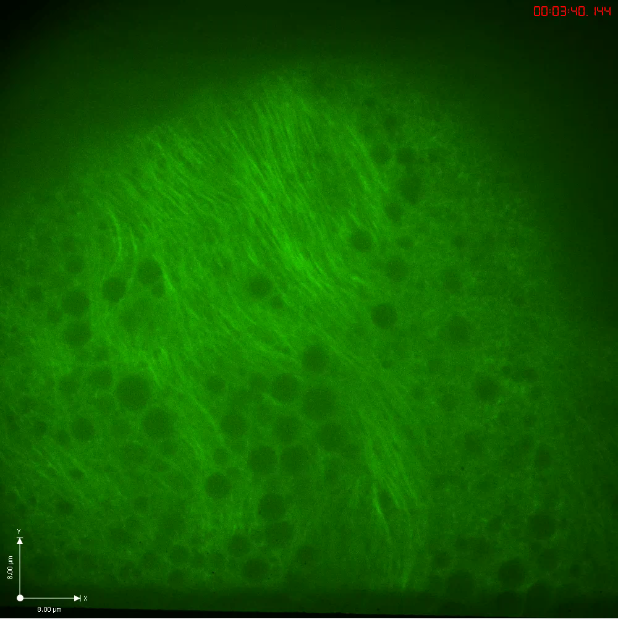
\includegraphics[width=\hsize]{fast.png}
\caption{ 
An image taken with a two photon microscope of a \emph{Drosophila} ooctye during fast streaming. The Oocyte was treated so that the microtubules would fluoresce and traces of them can be seen. In the regions of fast fluid motion, the microtubules can be seen to align with the direction of the fluid motion. Image care of Bill Saxton et. al.
}
\label{fig:biostream}
\end{center}
\end{figure}

We have previously shown that the motions of the microtubules is potentially consistent with the simple model of kinesin driven impellers in a pre-existing flow field. 
We still need to determine if a large group of microtubules are capable of spontaneously generating such a flow field.
However, since the microtubules align with a local flow field and then, once aligned, they contribute to that flow, it believable that a type of field amplification occurs.
Essentially, the long range interaction through the fluid could bring about a transition to a phase of long range order.

When the simulation is run with a small number of microtubules placed with their anchors near each other (less than the buckling length), short range correlation almost always emerges.
Using a random walk starting condition, the microtubules initially fall into seemingly independent circular solutions similar to those in the single microtubule case.
However, after a few periods of revolution the microtubules eventually collapse into one circular solution, as seen in Fig. \ref{fig:fourpoly}

\begin{figure}[htp]
\begin{center}
(a)
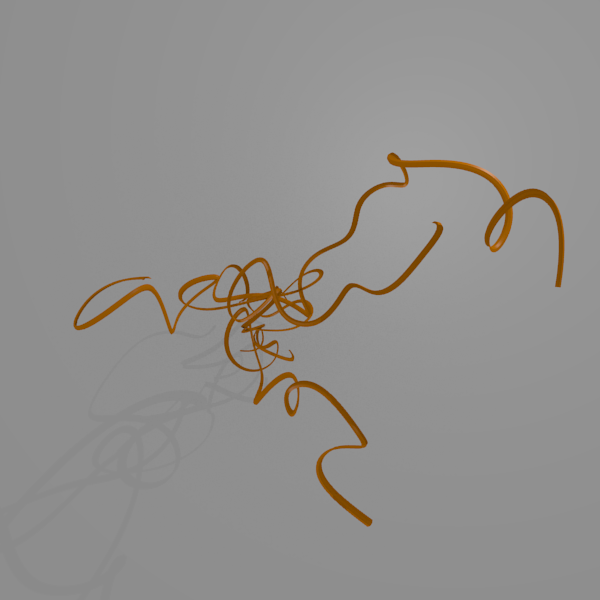
\includegraphics[width=0.45\hsize]{start.png}
(b)
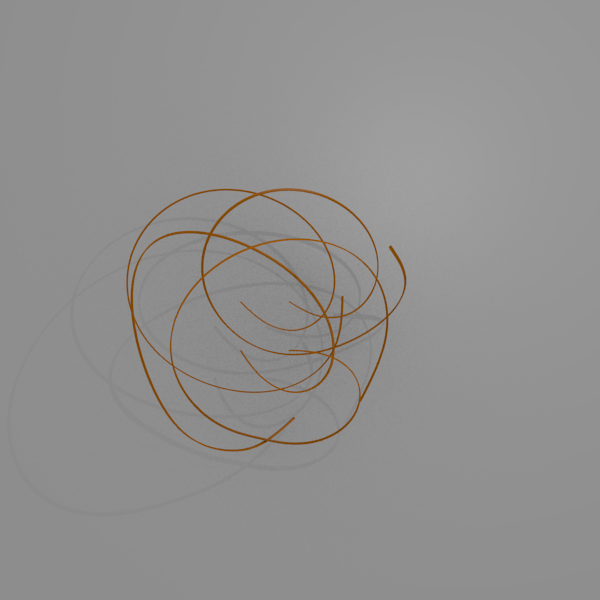
\includegraphics[width=0.45\hsize]{circ.png}
(c)
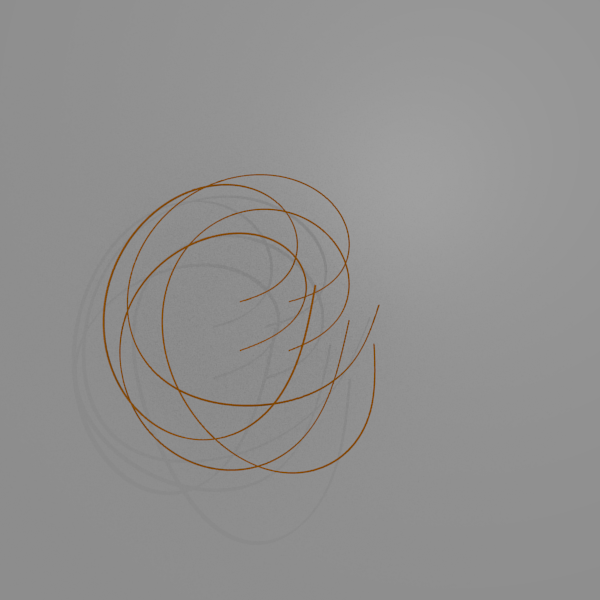
\includegraphics[width=0.45\hsize]{corr.png}
\caption{
(a)
A typical starting configuration of four microtubules, with $R_s = 2$ and $h = 2$. The apparent thickness is an artifact of the display method.
(b)
After a short time, the microtubules fall into individual circular solutions, with some correlation
(c)
After a few revolutions, all of the microtubules collapse into correlated circles.
}
\label{fig:fourpoly}
\end{center}
\end{figure}

While this correlation is a promising feature, it will not be enough to produce a long range directed flow field due to the circular nature of the motion.
In order to sustain linear streaming, the forces transmitted to any one microtubule from the rest of the system need to be stronger than the local kickback force from the kinesin motors.
A small number of microtubules will not be able to achieve this, so more need to be added to the simulation.

\subsection{Microtubule Patches}
In order to attain linear streaming in our simulation, we include a much larger group of microtubules.
These microtubules are placed with their anchor points in a square grid, and then some small random jitter is applied within the plane to their positions.
The random noise is added in order to suppress periodic lattice effects, which shouldn't be present in the cell.
Once the anchor points are chosen, the microtubules are initialized with a random walk biased slightly in the positive z direction to avoid problems caused by starting in the hard wall.
Any configuration that penetrated the wall was rejected.
Due to the random nature of the initial conditions, the microtubules often start with high curvatures.
This causes the first few steps of the simulation to be dominated by the microtubules rapidly relaxing to their more typical curvature.
This artifact of the somewhat artificial initial conditions shouldn't be relevant to the actual biological system, so these steps are generally not shown.
The forces that cause this relaxation are quite high, and occasionally they could cause the microtubules to break through the hard wall. 
This most often results in a divergence due to the hard wall Oseen tensor having odd behavior for negative z values.
Initial conditions that lead to this effect are also rejected.
A typical initialized patch is shown in Fig. \ref{fig:patchstart}

\begin{figure}[htp]
\begin{center}
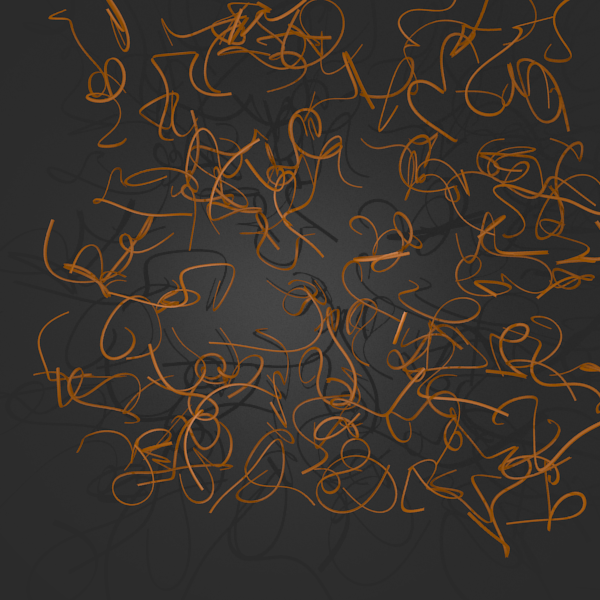
\includegraphics[width=\hsize]{fastsim.png}
\caption{ 
A typical starting configuration for a microtubule patch, viewed from directly above the plane.
}
\label{fig:patchstart}
\end{center}
\end{figure}

\subsection{Linear Streaming with Microtubule Patches}
There are a fairly wide range of parameters for which, regardless of the random initialization, the microtubule patch will self organize into a stable directed flow.
An example of this configuration can be seen in Fig. \ref{fig:streamline}

\begin{figure}[htp]
\begin{center}
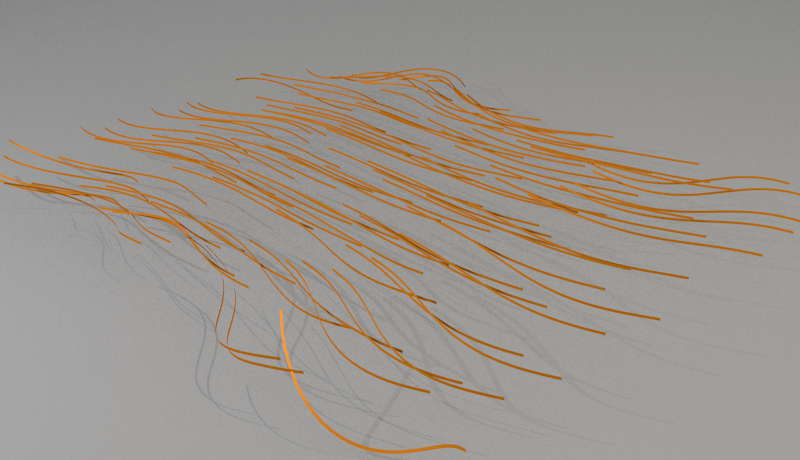
\includegraphics[width=\hsize]{streamline.png}
\caption{ 
A typical configuration after correlation, viewed from an angle to better show the planar nature of the solution. The microtubules on the edges of the patch can be seen to execute a helical pattern reminiscent of the single microtubule dynamics.
}
\label{fig:streamline}
\end{center}
\end{figure}

The length of time needed for the patch to reach this linear streaming phase can vary based on the parameters of the simulation, but in general it will be within a few periods of the single microtubule rotation.
During this correlation time, smaller sub regions of extended microtubules appear.
These sub regions can slowly rotate as a unit, and tend to cause more microtubules to correlate along with them as they pass nearby.
Once established, the linear streaming regions are stable and settle into a single direction.

It is important to re-emphasize that there is no externally imposed fluid motion in this simulation, and that the linear configuration is brought about by the fluid interactions between the microtubules.
The direction chosen for streaming is dependent on the exact nature of the random initial conditions, which are not guaranteed to be perfectly isotropic.
The spontaneous generation of this ordered phase will cause some aspects of the resulting system, such as the direction of the resulting global flow field, to depend sensitively on the initial conditions of the system.
However, many properties of the system in this phase, such as the flow speed and characteristic oscillation frequencies, should be independent of the initial conditions.
As long as the microtubules are essentially at rest in a steady state, the fluid velocity should be determined by the analysis from \ref{eq:mfflowlimit}; as a fraction of the impeller velocity given by $a/(a+d)$.

\subsection{Chaotic Solutions}
For some ranges of input parameters, the system will not manage to set up the fast linear streaming phase.
When the fluid interaction forces are not enough too overcome the kinesin reaction force, the microtubules will buckle and begin rotating around their anchor points.
Even though the hydrodynamic interaction is not strong enough to force a straight line solution, it can still cause the rotational solutions to correlate with each other, much like in the case of just a few microtubules.
Regions of correlated microtubules can develop, as see in Fig. \ref{fig:noodles}
The dynamic correlations found in this phase might include large numbers of microtubules, but rarely include the anchor points.
These masses of loose microtubule ends tend to flow back along their length, and as such represent very little  long range fluid motion.

\section{Conditions for Linear Streaming}
Not all microtubule patches will reach the linear streaming phase from a random initial condition.
There are ranges of parameters for which the system will only exhibit short range correlation, often in the same manner as the systems with only a few microtubules.
In these cases the forces from the fluid interaction are not strong enough to overcome the local kinesin reaction force, and the microtubules buckle and rotate around their anchor points.

\subsection{Effects of the wall}
The hard wall serves to damp out fluid motion near its surface due to its strong interaction with the fluid viscosity. 
This is seen in the interaction tensor as a negative force mirrored across the wall, opposing the motion of the true force above it.
One can imagine that, much like the case in electromagnetism, these mirror forces could form some sort of dipolar arrangement. 
This arrangement would have faster falloff with distance and could easily interfere with the ability of the entire system of microtubules to correlate over large distances.
We can see this effect in the simulation by simply placing the microtubule patch at several distances from the wall while holding the other parameters fixed.
Fig. \ref{fig:walldist} shows a sequence of separate patches, each at different distances from the wall. 

\begin{figure}[htp]
\begin{center}
(a)
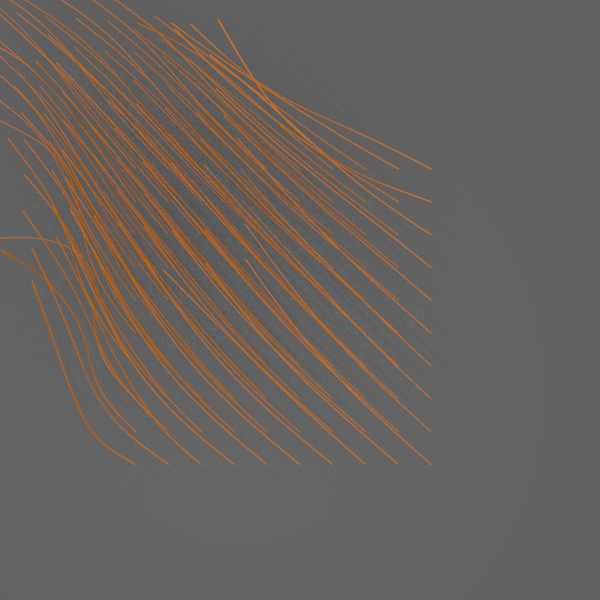
\includegraphics[width=0.45\hsize]{h5.png}
(b)
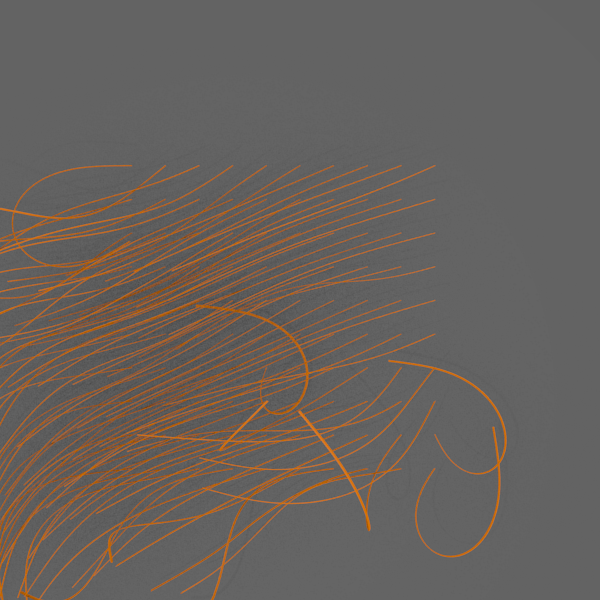
\includegraphics[width=0.45\hsize]{h3.png}
(c)
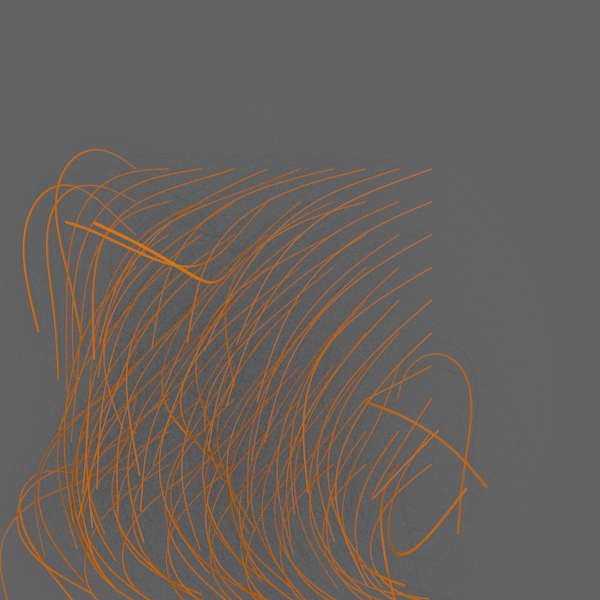
\includegraphics[width=0.45\hsize]{h2.png}
(d)
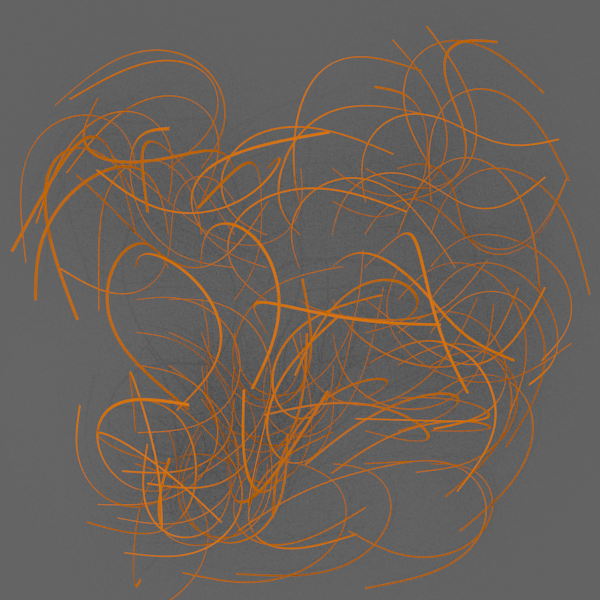
\includegraphics[width=0.45\hsize]{h1.png}
\caption{
(a-d) Configuration of microtubule patches after 200 simulation frames.
(a)Patch at $h=5$, shows strong directed streaming
(b)Patch at $h=3$, shows directed streaming, but with more loose edges
(c)Patch at $h=2$, shows directed streaming, but still "waves" and is not as straight
(d)Patch at $h=1$, shows no directed streaming, only correlation in circular motions
}
\label{fig:walldist}
\end{center}
\end{figure}

At large distances, the patches reach the linear streaming phase from the random initial state quite rapidly(within only a few rotation periods). 
As the distance from the wall is decreased, the time the system takes to reach the linear streaming state increases.

Eventually, the wall decreases the interaction strength significantly enough that the nucleation of the linear streaming regions cannot occur.
At these distances, the microtubules will often still correlate, but don't manage to achieve the straight line configuration.

% \subsection{Changing $R_b$}
% The characteristic buckling length is one of the primary length scales of the microtubule system, and unsurprisingly plays a key role in determining the phase of correlation the system will tend toward.

\subsection{Relative Viscosity}
One can also vary the viscosity of the fluid in this system.
As can be seen from Eq. \ref{eq:discretesum}, there is a global factor of $\mu^{-1}$ on all of the driving force terms.
Changing the viscosity will then inversely effect the fluid velocity field from the any given set of forces.
At first, it might seem that this would only cause a change in the overall timescale of the dynamics, but that turns out to be not quite true.
The motion of the microtubule itself is given by Eq. \ref{eq:discretelevel}, which includes a term only proportional to the kinesin walk speed.
If this speed remains unchanged, the effect of the kinesin forces will be scaled proportionately to the viscosity.

% \subsection{Tension Distribution During Correlated Streaming}
% Can has analytics?
% In the fast correlated streaming phase, the microtubules align and become largely straight.
% This configuration reduces the complexity of the system considerably, as the microtubules become largely stationary.
% In addition, the stiffness force term will vanish from the bulk of the microtubules.

\subsection{Hysterisus of Streaming}
Because it is a self reinforcing effect, the fast streaming behavior could very easily depend on the initial configuration of the microtubules. 
For instance, it is believable that a the system could be just barely able to support streaming with the microtubules aligned, but that such a system would be unable to spontaneously generate that alignment.
This divides our phase space up into additional regions.
One region is where the system always transitions to correlated streaming. One would imagine that this region would be one where interactions between microtubules are strong and long range compared to the other length scales in the system.
Another region is one where the system can support fast, correlated streaming, but may only reach it from certain classes of initial configurations. This region is obviously less robust if the intent is to achieve fast streaming.
A third region is one in which the system can never support fast correlated streaming. This would most likely be a region in which the interaction between microtubules is cut off at a range less than the typical spacing between microtubules.

We focus here primarily on the transition from disordered microtubules into correlated fast streaming.
This focus comes from the behavior of the cell during the stages before and after cytoplasmic streaming.
In the cell, microtubules are observed to be uncorrelated in the slow streaming phase, then during the fast streaming phase they are observed in correlated bundles.
The cell may undergo some change of internal parameters to cross the phase boundary from uncorrelated slow streaming to correlated fast streaming.


\section{Biologicaly Accesable Parameters for Streaming}
We have seen that many parameters can effect the ability of the model system to initiate linear fast streaming.
However, if the cell is indeed crossing this phase boundary in the transition from slow to fast streaming, it can only do so using parameters that can be changed in the cell in a relatively short timescale.
Some of the parameters can be artificially changed to try to isolate their effects.

Studies have been done to investigate the nature of the anchoring of the microtubules to the cell cortex \cite{WangRiechmann}.
These stuies show that in the stages of slow streaming, the microtubules are mostly anchor tightly against the sell cortex by think bundles of actin, another polymer used in the cytoskeleton.
These bundles are thought to hold the microtubule ends in a think layer very close to the cell wall, something which could prevent the production of correlated fast streaming.

After the fast streaming phase begins, the actin is no longer observed in tight bundles, but instead in a loose disorganized mesh.
In addition to this, the microtubules endpoints are observed to extend considerably farther in the cell, away from the cortex.
The distribution of endpoints is much wider, and extends two or three times farther from the cell wall.
This extension from the cortex is observed even in cell that have been modified to not have the Kinesin motors needed for fast streaming.
It would appear that the extension of microtubules away from the cell wall is not a side effect of the streaming.

This corresponds very closely to the simulation result that fast streaming can be suppressed by anchoring the microtubules tightly to the hard wall.
It is possible that the extension from the cortex is a mechanism to control the activation of fast streaming.
% Create the reference section using BibTeX:

%bibliography from Vacuum paper
\begin{thebibliography}{}
\bibitem{Hillenkamp} F. Hillenkamp (Editor), J. Peter-Katalinic (eds.). 
\bibitem{DeutschPolyVac} J.M. Deutsch, Phys. Rev. Lett. {\bf 99}, 238301 (2007).
\bibitem{Kleinert} H. Kleinert, Phys. Rev. B {\bf76}, 052202 (2007). 
\bibitem{mossa} A. Mossa, M. Pettini, and C. Clementi, Phys. Rev. E {\bf 74} 041805 (2006).

\bibitem{DeutschCerf} J.M. Deutsch, arXiv:1003.0944v2 
\bibitem{Taylor} M. P. Taylor, K. Isik and J. Luettmer-Strathmann,  Phys. Rev. E {\bf 78}, 051805  (2008).
\bibitem{DeutschExactVac} J.M. Deutsch, Phys. Rev. E {\bf 77}, 051804 (2008).
\bibitem{KleinertBook} H. Kleinert, ``Path Integrals in Quantum Mechanics, Statistics, Polymer Physics, and Financial Markets" Freie Universitat Berlin, Germany
\bibitem{laliena} V Laliena, Phys. Rev. E {\bf 59}, 4786 (1999).
\bibitem{feynman} R. P. Feynman, Statistical Mechanics: A Set of Lectures, Westview Press; 2nd Edition (1998)
\bibitem{SethnaBookKelvinFriction} J.P. Sethna ``Statistical Mechanics Entropy, Order
\bibitem{DeGennesBook} P.G. de Gennes ``Scaling Concepts in Polymer Physics" Cornell University Press (1985).
\bibitem{FPU} E. Fermi, J. Pasta, and S. Ulam, {\em Studies of nonlinear problems} 
(Los Alamos Document LA-1940, 1955).
\bibitem{BermanIzrailev} For a review see G.P. Berman and F.M. Izrailev, Chaos



%Bibliography from Mixing paper

\bibitem{SerbusSaxton} L.R. Serbus, B.J. Cha, W.E. Theurkauf, and  W.M. Saxton, 
``Dynein and the actin cytoskeleton control kinesin-driven cytoplasmic streaming in Drosophila oocytes."  Development {\bf 132},  3743-3752 (2005).
\bibitem{Movie13} See ref. \cite{SerbusSaxton} \href{http://www.ncbi.nlm.nih.gov/pmc/articles/PMC1534125/bin/NIHMS11364-supplement-Movie_13.mov}{Movie 13}.
\bibitem{LubyPhelps} K. Luby-Phelps, ``Cytoarchitecture and physical properties of cytoplasm: volume, viscosity, diffusion, intracellular 
surface area." Int. Rev. Cytol. {\bf 192} 189–221 (2000).
fluorescence redistribution after photobleaching." Journal of Cell Biology.  {\bf 99} 2165-2174 (1984). 
\bibitem{Squires} T. M. Squires and S. R. Quake, ``Microfluidics: Fluid physics at the nanoliter scale."
Rev. Mod. Phys., {\bf  77} 977-1026  (2005)
\bibitem{Aref} H. Aref,  ``Stirring by chaotic advection." J Fluid Mech. {\bf 143}, 1-21 (1984).
\bibitem{Aref2000} P. L. Boyland, H. Aref and M. A. Stremler, ``Topological fluid mechanics of stirring" J. Fluid Mech.  {\bf 403}  277-304 (2000),
\bibitem{Thurston} W. Thurston,  ``On the geometry and dynamics of diœmorphisms of surfaces", Bull. Am. Math.
Soc. {\bf 19}, 417-431 (1988).
\bibitem{Fathi} A. Fathi, F. Laudenbach, and V Poenaru,  ``Travaux de Thurston sur les surfaces." Asterique,
{\bf 66} (Seminaire Orsay) (1979).
\bibitem{Handel} M. Handel, ``Global shadowing of pseudo-Anosov homeomorphisms." Ergod. Theor. Dyn. Syst.
{\bf 5}, 373-377 (1985).
\bibitem{BergRandomWalksinBiology} Berg H. C. Random Walks in Biology (Princeton University Press, Princeton, NJ, 1983). 
\bibitem{SvobodaBlock} K. Svoboda and S. M. Block, ``Force and velocity measured for single kinesin molecules." Cell {\bf 77}, 773-784 (1994).
\bibitem{MeyhoferHoward} E. Meyh\"ofer and J. Howard,  ``The force generated by a single kinesin
molecule against an elastic load." Proc. Natl. Acad Sci. USA. {\bf 92} 574-578 (1995).
\bibitem{ChaSerbus} B J Cha, L R Serbus, B S Koppetsch, W E Theurkauf, 
``Kinesin I-dependent cortical exclusion restricts pole plasm to the oocyte posterior." Nat Cell Biol. {\bf 4} 592 (2002).
\bibitem{WangRiechmann} Y.  Wang and V. Riechmann, ``Microtubule anchoring by cortical actin bundles prevents streaming of the oocyte cytoplasm"
{\bf 125} 142-152 (2008).
\bibitem{Seeger}  M. A. Seeger and  S.  E. Rice, ``Microtubule-associated Protein-like Binding of the Kinesin-1 Tail to Microtubules", J. Biol. Cheme. {\bf 285}
8155-8162 (2010).
\bibitem{SupplMovies} The movies can be seen \href{http://physics.ucsc.edu/~josh/MTsim_videos/}{here}.
\bibitem{Kessler} D. A. Kessler, J. Koplik, H. Levine, ``Geometrical models of interface evolution. III. Theory of dendritic growth"  Phys. Rev. A {\bf 31}  1712 (1985).
\bibitem{Barbieri} A. Barbieri, D. C. Hong, J. S. Langer, ``Velocity selection in the symmetrical model of dendritic crystal growth." 
Phys. Rev. A {\bf 35} 1802 (1987).
\bibitem{SupplMat} J.M Deutsch, M. E.  Brunner, and W.M. Saxton, ``Analysis of microtubule motion due to drag from kinesin walkers" to be published.
\bibitem{Felgner} H. Felgner, R. Frank and M. Schliwa, ``Flexural rigidity of microtubules measured with the use of optical tweezers",
J. Cell Science 109, 509 (1996).
\bibitem{GittesRigidity} Gittes, F., B. Mickey, J. Nettleton, and J. Howard. 1993. ``Flexural rigidity
of microtubules and actin filaments measured from thermal fluctuations in shape." J. Cell Biol. 120:923-934.
\bibitem{YinStossel} H. L. Yin and T. P. Stossel, ``Control of cytoplasmic actin gel−sol transformation by gelsolin, a calcium-dependent regulatory protein"
Nature {\bf 281}, 583-586 (1979) 
\bibitem{Kennedy} J. R. Kennedy and K. E. Duckett, ``The study of ciliary frequencies with an optical spectrum analysis system",
Experimental Cell Research {\bf 135} 147 (1981).
\bibitem{ValeSchnappEtAl} R.D. Vale, B.J.  Schnapp, T.S. Reese, and M.P.  Sheetz,``Identification of a novel force-generating protein, kinesin, involved in microtubule-based motility"   Cell 40, 559-569 (1985).
\bibitem{MaloneyHerskowitzKoch} A. Maloney, L. J. Herskowitz and S. J. Koch, ``Effects of surface passivation on gliding motility assays""
Nature Precedings \href{http://precedings.nature.com/documents/4469/version/2}{hdl:10101/npre.2010.5278.1} (2010).
\bibitem{MaloneyKochVideo} Video is available at \href{http://www.kochlab.org/}{http://www.kochlab.org/} and\\ 
\href{http://www.youtube.com/watch?v=y0QCkObJIto}{http://www.youtube.com/watch?v=y0QCkObJIto}
\bibitem{KochLab} See the \href{http://openwetware.org/wiki/Koch_Lab}{Koch Lab Web Page}. 
\bibitem{OpenNotebookScience} See the wikipedia page on \href{http://en.wikipedia.org/wiki/Open_Notebook_Science}{Open Notebook Science}.



%Bibliography from Single Chain Paper
\bibitem{DeutschBrunnerSaxton} J.M. Deutsch, M.E. Brunner, and W. M. Saxton,
``The mechanics of a microscopic mixer: microtubules and cytoplasmic streaming in Drosophila oocytes", arXiv:1101.2225v1 [q-bio.SC] (2011).
\bibitem{CushmanBates} R. H. Cushman and L. M. Bates, ``Global aspects of classical integrable systems" Ch. IV, Birkh\"auser Basel, Boston, Berlin (1997).
\bibitem{Kessler} D. A. Kessler, J. Koplik, H. Levine, ``Geometrical models of interface evolution. III. Theory of dendritic growth"  Phys. Rev. A {\bf 31}  1712 (1985).
\bibitem{Barbieri} A. Barbieri, D. C. Hong, J. S. Langer, ``Velocity selection in the symmetrical model of dendritic crystal growth." 
Phys. Rev. A {\bf 35} 1802 (1987).
\bibitem{DeutschElectrophoresisScience} J. M Deutsch, Science ``Theoretical Studies of DNA During Gel electrophoresis." {\bf 240} 922-924 (1988).   
\bibitem{DeutschMadden}  J.M. Deutsch and TM. Madden,  ``Theoretical Studies of DNA During Gel electrophoresis." J Chem. Phys. {\bf 90} 2476-2485 (1989).
\bibitem{DeutschCerfFriction} J.M. Deutsch ``Internal dissipation of a polymer" Phys. Rev. E {\bf 81}, 061804/(16) (2010).
\bibitem{ValeSchnappEtAl} R.D. Vale, B.J.  Schnapp, T.S. Reese, and M.P.  Sheetz,``Identification of a novel force-generating protein, kinesin, involved in microtubule-based motility"   Cell 40, 559-569 (1985).
\bibitem{GoldsteinTuvalvandeMeentPNAS} R.E. Goldstein, I. Tuval, and J.W. van de Meent, ``Microfluidics of cytoplasmic streaming and its
implications for intracellular transport" Proc. Nat. Acad. Sci.,  {\bf 105}, 3663-3667 (2008).
\bibitem{GoldsteinTuvalvandeMeentPRL} R.E. Goldstein, I. Tuval, and J.W. van de Meent, 
``Nature’s Microfluidic Transporter: Rotational Cytoplasmic Streaming at High P{\'e}clet Numbers"
Phys. Rev. Lett. {\bf 101}, 178102(1-4) (2008)
\bibitem{MeentSedermanGladdenGoldstein} J.W. Van de Meent, A. J. Sederman, L. F. Gladden and R. E. Goldstein,
``Measurement of cytoplasmic streaming in single plant cells by magnetic resonance velocimetry"
J. Fluid Mech. {\bf 642},  5-14 (2010).
\bibitem{VerchotLubiczGoldstein}
J. Verchot-Lubicz  and R. E. Goldstein, ``Cytoplasmic streaming enables the distribution of molecules
and vesicles in large plant cells" Protoplasma {\bf 240} 99-107 (2010) 
\bibitem{WangRiechmann}
Ying Wang and Veit Riechmann, ``Microtubule anchoring by cortical actin bundles prevents streaming of the oocyte cytoplasm" Mechanisms of Developement {\bf 125} 142-152 (2007)
\end{thebibliography}

\end{document}
